% !TEX program = xelatex
% !TEX root = main.tex

% !TEX root = main.tex

% =============================
\documentclass[12pt,a4paper]{report}

% --- Font (Times New Roman asli) ---
\usepackage{fontspec}
\setmainfont{Times New Roman}[Ligatures=TeX,Renderer=Basic]

\usepackage[american,indonesian]{babel}

\usepackage{csquotes}
\usepackage[style=apa,backend=biber]{biblatex}
\addbibresource{references.bib}

% --- MAP bahasa indonesian ke mapping 'american-apa' yang tersedia ---
\DeclareLanguageMapping{indonesian}{american-apa}

% --- Override label bibliografi ke Bahasa Indonesia ---
\DefineBibliographyStrings{indonesian}{%
  bibliography = {DAFTAR PUSTAKA},
  references = {DAFTAR PUSTAKA},
  and          = {\&},
}

% Pilih bahasa tampilan dokumen jadi indonesian
\AtBeginDocument{\selectlanguage{indonesian}}

% --- Margin ---
\usepackage{geometry}
\geometry{
  a4paper,
  left=4cm,
  right=3cm,
  top=4cm,
  bottom=3cm
}

% --- Spasi 1.5 ---
\usepackage{setspace}
\onehalfspacing

% --- Paragraf (indentasi) ---
\usepackage{indentfirst}
\setlength{\parindent}{1cm}
\setlength{\parskip}{0pt}

% --- Matematika & fisika ---
\usepackage{amsmath,amssymb,amsfonts,mathtools}
\usepackage{physics}
\usepackage{bm}
\usepackage{tensor}
\usepackage{siunitx}

% --- Gambar & grafik ---
\usepackage{graphicx}
\usepackage{caption}
\usepackage{subcaption}
\usepackage{float}

% --- Tabel ---
\usepackage{booktabs}
\usepackage{multirow}
\usepackage{array}

% --- Listing kode Python ---
\usepackage{listings}
\usepackage{xcolor}

\definecolor{codebg}{RGB}{245,245,245}
\definecolor{codegreen}{RGB}{0,128,0}
\definecolor{codegray}{RGB}{128,128,128}
\definecolor{codepurple}{RGB}{128,0,128}

\lstdefinestyle{pythonstyle}{
  backgroundcolor=\color{codebg},
  basicstyle=\ttfamily\small,
  breaklines=true,
  captionpos=b,
  commentstyle=\color{codegreen},
  keywordstyle=\color{codepurple}\bfseries,
  stringstyle=\color{red!70!black},
  numberstyle=\tiny\color{codegray},
  numbers=left,
  numbersep=5pt,
  frame=single,
  rulecolor=\color{black!30},
  tabsize=4,
  language=Python,
  showstringspaces=false,
}
\lstset{style=pythonstyle}

% --- Hyperlink & referensi ---
\usepackage[hidelinks]{hyperref}
\usepackage{cleveref}

% --- Penomoran persamaan per bab ---
\numberwithin{equation}{chapter}

% --- Enumerate custom ---
\usepackage{enumitem}

% --- Format judul bab ---
\usepackage{titlesec}

\renewcommand{\thechapter}{\arabic{chapter}}
\renewcommand{\thesection}{\thechapter.\arabic{section}}
\renewcommand{\thesubsection}{\thesection.\arabic{subsection}}

\titleformat{\chapter}[display]
  {\normalfont\centering\bfseries\normalsize}
  {\MakeUppercase{BAB \Roman{chapter}}}
  {0pt}
  {\vspace{1ex}\MakeUppercase}
\titlespacing*{\chapter}{0pt}{0pt}{20pt}

\titleformat{\section}
  {\normalfont\bfseries\normalsize}
  {\thesection}{1em}{}
\titlespacing*{\section}{0pt}{12pt}{6pt}

\titleformat{\subsection}
  {\normalfont\bfseries\normalsize}
  {\thesubsection}{1em}{}
\titlespacing*{\subsection}{0pt}{10pt}{4pt}

\usepackage[none]{hyphenat}
\sloppy


% --- Informasi skripsi ---
\title{\textbf{Kajian Analitik dan Penyelesaian Numerik Efek Lense-Thirring pada Metrik Kerr: Studi Kasus Gravity Probe B}}
\author{Pramudya Jesril Pratama}
\date{\today}

\begin{document}

% ---------- Judul (titlepage) ----------
\maketitle

% ---------- Penomoran HALAMAN MUKA: Roman kecil ----------
\pagenumbering{roman}

% !TEX root = ../main.tex

\chapter*{Abstrak}
\addcontentsline{toc}{chapter}{Abstrak}

Relativitas Umum memprediksi bahwa massa berotasi menginduksi penyeretan kerangka acuan inersia lokal, yang dikenal sebagai efek Lense-Thirring atau \textit{frame-dragging}.
Efek ini telah dikonfirmasi secara eksperimental oleh misi \textit{Gravity Probe B} (GP-B) dengan hasil pengukuran sebesar $37{,}2 \pm 7{,}2$ milliarcsecond per tahun (mas/yr) untuk presesi \textit{frame-dragging} dan $6602 \pm 18$ mas/yr untuk presesi geodesik.
Penelitian ini menyajikan kajian analitik terhadap persamaan geodesik dan transportasi paralel tensor spin pada metrik Kerr, serta penyelesaian numeriknya untuk konfigurasi orbit Bumi.
Metrik Kerr dalam koordinat Boyer-Lindquist diturunkan secara eksplisit dalam bentuk matriks $4 \times 4$, dan simbol-simbol Christoffel yang relevan dihitung untuk memperoleh persamaan gerak.
Lagrangian metrik Kerr digunakan untuk menurunkan persamaan geodesik melalui metode Euler-Lagrange, yang kemudian direduksi menjadi sistem persamaan diferensial biasa orde satu.
Aproksimasi medan lemah diterapkan untuk memperoleh ekspresi analitik laju presesi Lense-Thirring $\Omega_{\text{LT}} \approx 2GJ/(c^2 r^3)$.
Sistem persamaan diferensial yang dihasilkan diselesaikan secara numerik menggunakan metode Runge-Kutta orde empat yang diimplementasikan dalam Python.
Hasil simulasi menunjukkan laju presesi geodesik sebesar $\sim\!6600$ mas/yr dan \textit{frame-dragging} sebesar $\sim\!37$ mas/yr, konsisten dengan data eksperimen GP-B dalam batas galat pengukuran.
Analisis kestabilan numerik dan sensitivitas terhadap parameter rotasi Bumi turut disajikan untuk memvalidasi keandalan metode komputasi yang digunakan.

\vspace{1em}
\noindent\textbf{Kata Kunci:} Relativitas Umum, Metrik Kerr, Efek Lense-Thirring, \textit{Frame-Dragging}, Presesi Geodesik, Gravity Probe B, Penyelesaian Numerik.


\tableofcontents
\listoffigures
\listoftables

% ---------- Isi utama: penomoran Arab ----------
\cleardoublepage
\pagenumbering{arabic}
\setcounter{page}{1}

% !TEX root = ../main.tex

\chapter{Pendahuluan}
\label{chap:pendahuluan}

% ============================================================
\section{Latar Belakang}
\label{sec:latar-belakang}

Teori Relativitas Umum (\textit{General Relativity}, GR) yang dirumuskan oleh Einstein pada tahun 1915 merupakan teori gravitasi yang mendeskripsikan interaksi gravitasi sebagai manifestasi kelengkungan ruang-waktu empat dimensi. Dalam kerangka ini, distribusi massa dan energi menentukan geometri ruang-waktu melalui persamaan medan Einstein $G_{\mu\nu} = \frac{8\pi G}{c^4}\, T_{\mu\nu}$, di mana $G_{\mu\nu}$ adalah tensor Einstein dan $T_{\mu\nu}$ adalah tensor energi-momentum \parencite{Einstein1916GR, Misner1973Gravitation}. Gerak benda uji dalam ruang-waktu melengkung ditentukan oleh persamaan geodesik yang bergantung pada simbol Christoffel $\Gamma^\mu_{\nu\rho}$, yang diturunkan dari tensor metrik $g_{\mu\nu}$ \parencite{Carroll2004SpacetimeGeometry}.

Salah satu konsekuensi penting dari GR adalah prediksi bahwa massa berotasi tidak hanya melengkungkan ruang-waktu, tetapi juga menyeret kerangka acuan inersia lokal di sekitarnya. Efek ini dikenal sebagai \textit{frame-dragging} atau efek Lense-Thirring, yang pertama kali diprediksi secara teoretis oleh \textcite{Lense1918LenseThirring}. Secara matematis, efek ini muncul dari suku campuran $g_{t\phi}$ pada metrik Kerr yang mendeskripsikan ruang-waktu di sekitar massa berotasi \parencite{Kerr1963KerrMetric}. Selain efek Lense-Thirring, GR juga memprediksi adanya presesi geodesik (\textit{geodetic precession} atau efek de Sitter), yaitu perubahan orientasi giroskop akibat geraknya melalui ruang-waktu yang melengkung oleh massa statis \parencite{Carroll2004SpacetimeGeometry, Will2014Confrontation}.

Kedua efek ini telah diverifikasi secara eksperimental melalui misi \textit{Gravity Probe B} (GP-B) yang diluncurkan oleh NASA pada tahun 2004. Misi ini menggunakan empat giroskop kuarsa berpresisi tinggi dalam orbit polar di sekitar Bumi pada ketinggian $\sim$642~km. Hasil pengukuran GP-B menunjukkan laju presesi geodesik sebesar $6602 \pm 18$ milliarcsecond per tahun (mas/yr) dan laju presesi \textit{frame-dragging} sebesar $37{,}2 \pm 7{,}2$~mas/yr, keduanya konsisten dengan prediksi GR \parencite{Everitt2011GravityProbeB}.

Meskipun hasil eksperimen GP-B telah dikonfirmasi, kajian analitik terhadap proses derivasi matematis yang mendasari prediksi tersebut tetap memiliki nilai penting. Prediksi laju presesi Lense-Thirring memerlukan serangkaian langkah derivasi yang meliputi: (i)~penulisan eksplisit tensor metrik Kerr dalam koordinat Boyer-Lindquist, (ii)~perhitungan simbol Christoffel dari komponen-komponen metrik, (iii)~penurunan persamaan geodesik melalui metode Lagrangian, (iv)~formulasi persamaan transportasi paralel tensor spin, dan (v)~reduksi ke aproksimasi medan lemah untuk memperoleh ekspresi analitik laju presesi. Setiap langkah tersebut melibatkan operasi kalkulus tensor yang tidak trivial dan jarang disajikan secara lengkap dalam satu kajian terpadu \parencite{Carroll2004SpacetimeGeometry, Schutz2009FirstCourse}.

Di sisi lain, persamaan diferensial yang dihasilkan dari derivasi tersebut bersifat sangat nonlinier, sehingga penyelesaian analitik eksak hanya dimungkinkan pada kasus-kasus tertentu dengan simetri tinggi. Untuk konfigurasi orbit yang realistis, diperlukan penyelesaian numerik menggunakan metode seperti Runge-Kutta orde empat atau integrator simplektik \parencite{Butcher2016NumericalMethods, Hairer2006GeometricIntegration}. Implementasi numerik ini dapat dilakukan dengan bantuan pustaka komputasi Python seperti \texttt{EinsteinPy} dan \texttt{SciPy} \parencite{Bapat2020EinsteinPy, SciPy2020}.

Berdasarkan latar belakang tersebut, penelitian ini menyajikan kajian analitik terhadap persamaan geodesik dan transportasi paralel tensor spin pada metrik Kerr, serta penyelesaian numerik sistem persamaan diferensial yang dihasilkan untuk konfigurasi orbit Bumi. Hasil komputasi numerik kemudian dibandingkan dengan data eksperimen GP-B sebagai validasi konsistensi antara derivasi analitik dan pengamatan eksperimental.

% ============================================================
\section{Batasan Masalah}
\label{sec:batasan-masalah}

Penelitian ini dibatasi pada hal-hal berikut:
\begin{enumerate}[label=\arabic*)]
    \item Kajian dilakukan dalam kerangka Relativitas Umum dengan menggunakan metrik Kerr sebagai representasi ruang-waktu di sekitar Bumi yang berotasi. Metrik Schwarzschild digunakan sebagai kasus batas non-rotasi ($a = 0$) untuk keperluan analisis sensitivitas.
    \item Model ruang-waktu dibatasi pada orbit di sekitar Bumi dengan mengabaikan pengaruh benda langit lain.
    \item Analisis difokuskan pada dua efek relativistik utama: presesi geodesik dan efek Lense-Thirring (\textit{frame-dragging}).
    \item Derivasi analitik dilakukan dalam kerangka kalkulus tensor. Penyelesaian numerik menggunakan metode Runge-Kutta yang diimplementasikan dalam Python.
    \item Penelitian bersifat kajian analitik-numerik, tanpa melibatkan pengamatan eksperimental langsung.
\end{enumerate}

% ============================================================
\section{Rumusan Masalah}
\label{sec:rumusan-masalah}

Berdasarkan latar belakang dan batasan masalah yang telah diuraikan, rumusan masalah dalam penelitian ini adalah sebagai berikut:
\begin{enumerate}[label=\arabic*)]
    \item Bagaimana menurunkan persamaan geodesik dan persamaan transportasi paralel tensor spin dari metrik Kerr melalui metode Lagrangian dan kalkulus tensor?
    \item Bagaimana mereduksi metrik Kerr ke dalam aproksimasi medan lemah untuk memperoleh ekspresi analitik laju presesi Lense-Thirring pada kasus Bumi?
    \item Bagaimana menyelesaikan sistem persamaan diferensial geodesik dan transportasi paralel spin secara numerik, serta memvalidasi hasilnya terhadap data eksperimen \textit{Gravity Probe B}?
\end{enumerate}

% ============================================================
\section{Tujuan Penelitian}
\label{sec:tujuan-penelitian}

Tujuan dari penelitian ini adalah sebagai berikut:
\begin{enumerate}[label=\arabic*)]
    \item Menurunkan persamaan geodesik dari Lagrangian metrik Kerr melalui persamaan Euler-Lagrange, serta merumuskan persamaan transportasi paralel tensor spin dalam bentuk matriks.
    \item Melakukan reduksi metrik Kerr ke aproksimasi medan lemah dan menurunkan ekspresi analitik laju presesi Lense-Thirring $\Omega_{\text{LT}} \approx 2GJ/(c^2 r^3)$ untuk konfigurasi Bumi.
    \item Menyelesaikan sistem persamaan diferensial yang diperoleh secara numerik menggunakan metode Runge-Kutta, dan membandingkan hasil komputasi dengan data pengukuran \textit{Gravity Probe B}.
\end{enumerate}

% ============================================================
\section{Manfaat Penelitian}
\label{sec:manfaat-penelitian}

Manfaat dari penelitian ini adalah sebagai berikut:
\begin{enumerate}[label=\arabic*)]
    \item Bagi ilmu pengetahuan: menyediakan kajian terpadu yang menjabarkan derivasi analitik efek Lense-Thirring dari metrik Kerr secara langkah demi langkah, mulai dari tensor metrik hingga ekspresi laju presesi, disertai verifikasi numerik.
    \item Bagi penulis: mengembangkan pemahaman mendalam di bidang kalkulus tensor, Relativitas Umum, dan metode penyelesaian numerik persamaan diferensial.
    \item Bagi akademis: menghasilkan dokumen referensi yang dapat digunakan sebagai bahan pembelajaran mengenai derivasi efek relativistik pada metrik Kerr dan implementasi komputasinya.
\end{enumerate}

% !TEX root = ../main.tex

\chapter{Tinjauan Pustaka}
\label{chap:tinjauan}

% ============================================================
\section{Relativitas Umum Einstein}
\label{sec:relativitas-umum}

Relativitas Umum (GR) mendeskripsikan gravitasi sebagai kelengkungan ruang-waktu empat dimensi yang ditentukan oleh distribusi massa dan energi. Hubungan antara geometri ruang-waktu dan sumber gravitasi dinyatakan oleh persamaan medan Einstein \parencite{Einstein1916GR}:
\begin{equation}
    R_{\mu\nu} - \frac{1}{2}\, R\, g_{\mu\nu} = \frac{8\pi G}{c^4}\, T_{\mu\nu},
    \label{eq:efe}
\end{equation}
di mana $R_{\mu\nu}$ adalah tensor Ricci, $R = g^{\mu\nu}R_{\mu\nu}$ adalah skalar kelengkungan, $g_{\mu\nu}$ adalah tensor metrik, dan $T_{\mu\nu}$ adalah tensor energi-momentum. Tensor Ricci diperoleh dari kontraksi tensor Riemann:
\begin{equation}
    R^\rho_{\ \sigma\mu\nu} = \partial_\mu \Gamma^\rho_{\nu\sigma}
    - \partial_\nu \Gamma^\rho_{\mu\sigma}
    + \Gamma^\rho_{\mu\lambda}\Gamma^\lambda_{\nu\sigma}
    - \Gamma^\rho_{\nu\lambda}\Gamma^\lambda_{\mu\sigma},
    \label{eq:riemann}
\end{equation}
dengan $R_{\mu\nu} = R^\rho_{\ \mu\rho\nu}$ \parencite{Carroll2004SpacetimeGeometry, Misner1973Gravitation}.

Gerak partikel bebas dalam ruang-waktu melengkung mengikuti lintasan geodesik, yaitu kurva yang memenuhi:
\begin{equation}
    \frac{d^2 x^\mu}{d\tau^2}
    + \Gamma^\mu_{\nu\rho}\,\frac{dx^\nu}{d\tau}\,\frac{dx^\rho}{d\tau} = 0,
    \label{eq:geodesic}
\end{equation}
di mana $\tau$ adalah waktu proper dan $\Gamma^\mu_{\nu\rho}$ adalah simbol Christoffel yang didefinisikan pada Persamaan~\eqref{eq:christoffel-def} \parencite{Schutz2009FirstCourse}.


% ============================================================
\section{Tensor Metrik dan Simbol Christoffel}
\label{sec:metrik-christoffel}

\subsection{Simbol Christoffel}
\label{subsec:christoffel-umum}

Simbol Christoffel jenis kedua $\Gamma^\mu_{\nu\rho}$ menggambarkan koneksi Levi-Civita pada manifold pseudo-Riemannian dan didefinisikan sebagai:
\begin{equation}
    \Gamma^\mu_{\nu\rho} = \frac{1}{2}\, g^{\mu\sigma}
    \left(
        \frac{\partial g_{\sigma\nu}}{\partial x^\rho}
      + \frac{\partial g_{\sigma\rho}}{\partial x^\nu}
      - \frac{\partial g_{\nu\rho}}{\partial x^\sigma}
    \right).
    \label{eq:christoffel-def}
\end{equation}
Simbol ini bersifat simetris terhadap dua indeks bawah, $\Gamma^\mu_{\nu\rho} = \Gamma^\mu_{\rho\nu}$, dan berjumlah paling banyak 40 komponen independen dalam ruang-waktu empat dimensi. Untuk metrik diagonal, banyak komponen bernilai nol, namun metrik Kerr memiliki suku campuran $g_{t\phi} \neq 0$ yang menghasilkan komponen Christoffel tambahan yang tidak trivial \parencite{Carroll2004SpacetimeGeometry}.


\subsection{Metrik Schwarzschild}
\label{subsec:metrik-schwarzschild}

Solusi Schwarzschild mendeskripsikan ruang-waktu di sekitar massa statis tak berotasi. Dalam koordinat bola $(t, r, \theta, \phi)$, elemen garisnya diberikan oleh \parencite{Schwarzschild1916Field}:
\begin{equation}
    ds^2 = \left(1 - \frac{r_s}{r}\right) c^2\,dt^2
         - \left(1 - \frac{r_s}{r}\right)^{-1} dr^2
         - r^2\, d\theta^2
         - r^2 \sin^2\!\theta\, d\phi^2,
    \label{eq:schwarzschild}
\end{equation}
dengan $r_s = 2GM/c^2$ adalah radius Schwarzschild. Metrik ini bersifat diagonal dan menghasilkan efek presesi geodesik, namun tidak mengandung efek \textit{frame-dragging} karena tidak adanya suku campuran $dt\,d\phi$.


\subsection{Metrik Kerr}
\label{subsec:metrik-kerr}

Metrik Kerr merupakan solusi eksak persamaan medan Einstein untuk massa berotasi tanpa muatan listrik, ditemukan oleh \textcite{Kerr1963KerrMetric}. Dalam koordinat Boyer-Lindquist $(t, r, \theta, \phi)$, elemen garisnya dapat dituliskan sebagai:
\begin{equation}
\begin{split}
    ds^2 &= \left(1 - \frac{r_s r}{\Sigma}\right) c^2\,dt^2
          + \frac{2\,r_s\, r\, a \sin^2\!\theta}{\Sigma}\; c\,dt\,d\phi
          - \frac{\Sigma}{\Delta}\, dr^2
          - \Sigma\, d\theta^2 \\
         &\quad - \left(r^2 + a^2 + \frac{r_s\, r\, a^2 \sin^2\!\theta}{\Sigma}\right)
           \sin^2\!\theta\, d\phi^2,
\end{split}
    \label{eq:kerr-line}
\end{equation}
dengan fungsi-fungsi bantu:
\begin{equation}
    \Sigma \equiv r^2 + a^2 \cos^2\!\theta, \qquad
    \Delta \equiv r^2 - r_s\, r + a^2,
    \label{eq:sigma-delta}
\end{equation}
di mana $r_s = 2GM/c^2$ dan $a = J/(Mc)$ adalah parameter rotasi spesifik, dengan $J$ menyatakan momentum sudut total massa pusat \parencite{Kerr1963KerrMetric, Carroll2004SpacetimeGeometry}.

Dengan menggunakan konvensi koordinat $x^\mu = (x^0, x^1, x^2, x^3) = (ct, r, \theta, \phi)$, tensor metrik Kerr $g_{\mu\nu}$ dapat dituliskan dalam bentuk matriks $4 \times 4$ sebagai:
\begin{equation}
    g_{\mu\nu} =
    \begin{pmatrix}
        1 - \dfrac{r_s r}{\Sigma} & 0 & 0 & \dfrac{r_s\, r\, a \sin^2\!\theta}{\Sigma} \\[12pt]
        0 & -\dfrac{\Sigma}{\Delta} & 0 & 0 \\[12pt]
        0 & 0 & -\Sigma & 0 \\[12pt]
        \dfrac{r_s\, r\, a \sin^2\!\theta}{\Sigma} & 0 & 0
        & -\!\left(r^2 + a^2 + \dfrac{r_s\, r\, a^2 \sin^2\!\theta}{\Sigma}\right)\sin^2\!\theta
    \end{pmatrix}.
    \label{eq:kerr-matrix}
\end{equation}

Beberapa sifat penting dari matriks metrik ini:
\begin{enumerate}[label=(\roman*)]
    \item Komponen $g_{t\phi} = g_{\phi t} = r_s\, r\, a \sin^2\!\theta\,/\,\Sigma$ tidak bernilai nol jika $a \neq 0$. Suku campuran inilah yang bertanggung jawab atas efek \textit{frame-dragging}.
    \item Pada limit $a \to 0$, matriks di atas tereduksi menjadi metrik Schwarzschild diagonal (Persamaan~\ref{eq:schwarzschild}).
    \item Komponen $g_{rr}$ memiliki singularitas koordinat pada $\Delta = 0$, yang terjadi pada horizon peristiwa.
\end{enumerate}

Metrik invers $g^{\mu\nu}$ diperlukan untuk menghitung simbol Christoffel. Dengan memanfaatkan struktur blok-diagonal ($2 \times 2$ pada sub-ruang $t$-$\phi$ dan diagonal pada $r$-$\theta$), komponen-komponen metrik invers diperoleh sebagai:
\begin{equation}
\begin{aligned}
    g^{tt} &= \frac{1}{\Delta}\left(r^2 + a^2 + \frac{r_s\, r\, a^2 \sin^2\!\theta}{\Sigma}\right), &\qquad
    g^{t\phi} &= \frac{r_s\, r\, a}{\Sigma\,\Delta}, \\[6pt]
    g^{rr} &= -\frac{\Delta}{\Sigma}, &\qquad
    g^{\theta\theta} &= -\frac{1}{\Sigma}, \\[6pt]
    g^{\phi\phi} &= -\frac{1}{\Delta\sin^2\!\theta}\left(1 - \frac{r_s\, r}{\Sigma}\right), &\qquad
    & \text{komponen lain} = 0.
\end{aligned}
    \label{eq:kerr-inverse}
\end{equation}


\subsection{Contoh Perhitungan Simbol Christoffel Metrik Kerr}
\label{subsec:christoffel-kerr-contoh}

Perhitungan simbol Christoffel untuk metrik Kerr menghasilkan sejumlah besar komponen yang tidak bernilai nol. Pada bagian ini disajikan derivasi eksplisit untuk tiga komponen representatif yang relevan dengan efek \textit{frame-dragging}.

\paragraph{Contoh 1: $\Gamma^t_{tr}$.}
Menggunakan Persamaan~\eqref{eq:christoffel-def} dengan $\mu = t$, $\nu = t$, $\rho = r$:
\begin{equation}
    \Gamma^t_{tr} = \frac{1}{2}\,g^{t\sigma}
    \left(\partial_r g_{\sigma t} + \partial_t g_{\sigma r} - \partial_\sigma g_{tr}\right).
\end{equation}
Karena metrik tidak bergantung pada $t$ (stasioner), suku $\partial_t g_{\sigma r} = 0$. Kontribusi non-nol berasal dari $\sigma = t$ dan $\sigma = \phi$:
\begin{equation}
    \Gamma^t_{tr} = \frac{1}{2}\,g^{tt}\,\partial_r g_{tt}
                  + \frac{1}{2}\,g^{t\phi}\,\partial_r g_{\phi t}.
    \label{eq:christoffel-ttr}
\end{equation}
Turunan parsial $\partial_r g_{tt}$ dan $\partial_r g_{t\phi}$ dapat dihitung dari Persamaan~\eqref{eq:kerr-matrix}. Sebagai contoh:
\begin{equation}
    \frac{\partial g_{tt}}{\partial r}
    = \frac{\partial}{\partial r}\left(1 - \frac{r_s\, r}{\Sigma}\right)
    = -r_s\,\frac{\Sigma - r(2r)}{\Sigma^2}
    = \frac{r_s(r^2 - a^2\cos^2\!\theta)}{\Sigma^2},
    \label{eq:dgtt-dr}
\end{equation}
mengingat $\partial_r \Sigma = 2r$. Substitusi ke Persamaan~\eqref{eq:christoffel-ttr} bersama dengan ekspresi $g^{tt}$ dan $g^{t\phi}$ dari Persamaan~\eqref{eq:kerr-inverse} menghasilkan:
\begin{equation}
    \Gamma^t_{tr} = \frac{r_s(r^2 - a^2\cos^2\!\theta)(r^2 + a^2)}{2\,\Sigma^2\,\Delta}
    + \frac{r_s^2\, r\, a^2\sin^2\!\theta\,(r^2 - a^2\cos^2\!\theta)}{2\,\Sigma^3\,\Delta}.
    \label{eq:gamma-ttr-result}
\end{equation}

\paragraph{Contoh 2: $\Gamma^\phi_{tr}$.}
Komponen ini menggambarkan kopling langsung antara gerak radial dan gerak azimut akibat rotasi sumber:
\begin{equation}
    \Gamma^\phi_{tr} = \frac{1}{2}\,g^{\phi\sigma}
    \left(\partial_r g_{\sigma t} + \partial_t g_{\sigma r} - \partial_\sigma g_{tr}\right).
\end{equation}
Dengan $\partial_t = 0$ dan kontribusi dari $\sigma = t$ serta $\sigma = \phi$:
\begin{equation}
    \Gamma^\phi_{tr} = \frac{1}{2}\,g^{\phi t}\,\partial_r g_{tt}
                     + \frac{1}{2}\,g^{\phi\phi}\,\partial_r g_{\phi t}.
    \label{eq:christoffel-phitr}
\end{equation}
Perhatikan bahwa $g^{\phi t} = g^{t\phi}$. Substitusi komponen metrik invers (Persamaan~\ref{eq:kerr-inverse}) dan turunan yang sesuai memberikan ekspresi dalam $r$, $\theta$, $\Sigma$, dan $\Delta$. Komponen ini bernilai nol pada limit $a \to 0$ (metrik Schwarzschild), yang menegaskan bahwa kopling $r$-$\phi$ murni berasal dari rotasi massa.

\paragraph{Contoh 3: $\Gamma^t_{\theta\phi}$.}
Komponen ini menunjukkan kopling antara gerak polar dan azimut melalui koordinat waktu:
\begin{equation}
    \Gamma^t_{\theta\phi} = \frac{1}{2}\,g^{t\sigma}
    \left(\partial_\phi g_{\sigma\theta} + \partial_\theta g_{\sigma\phi} - \partial_\sigma g_{\theta\phi}\right).
\end{equation}
Karena metrik tidak bergantung pada $\phi$ (simetri aksial) dan $g_{r\theta} = g_{r\phi} = 0$, maka:
\begin{equation}
    \Gamma^t_{\theta\phi} = \frac{1}{2}\,g^{tt}\,\partial_\theta g_{t\phi}
                          + \frac{1}{2}\,g^{t\phi}\,\partial_\theta g_{\phi\phi}.
    \label{eq:christoffel-tthetaphi}
\end{equation}
Turunan $\partial_\theta g_{t\phi}$ memerlukan:
\begin{equation}
    \frac{\partial g_{t\phi}}{\partial\theta}
    = \frac{\partial}{\partial\theta}
    \!\left(\frac{r_s\, r\, a\sin^2\!\theta}{\Sigma}\right)
    = \frac{r_s\, r\, a}{\Sigma^2}
    \left(2\Sigma\sin\theta\cos\theta + 2a^2\sin^3\!\theta\cos\theta\right),
\end{equation}
yang menunjukkan ketergantungan eksplisit pada sudut polar $\theta$. Komponen ini juga lenyap pada limit $a \to 0$.

Perhitungan lengkap seluruh komponen Christoffel metrik Kerr menghasilkan puluhan suku yang kompleks. Dalam praktik, perhitungan ini dapat diverifikasi dan dilakukan secara efisien menggunakan pustaka komputasi simbolik seperti \texttt{EinsteinPy} \parencite{Bapat2020EinsteinPy}.


% ============================================================
\section{Persamaan Geodesik}
\label{sec:persamaan-geodesik}

Lintasan partikel uji bermassa dalam ruang-waktu melengkung dapat diturunkan dari prinsip aksi minimal. Lagrangian untuk partikel pada metrik $g_{\mu\nu}$ diberikan oleh:
\begin{equation}
    \mathcal{L} = \frac{1}{2}\, g_{\mu\nu}\, \dot{x}^\mu\, \dot{x}^\nu,
    \label{eq:lagrangian}
\end{equation}
dengan $\dot{x}^\mu \equiv dx^\mu/d\tau$. Penerapan persamaan Euler-Lagrange,
\begin{equation}
    \frac{d}{d\tau}\frac{\partial\mathcal{L}}{\partial\dot{x}^\mu}
    - \frac{\partial\mathcal{L}}{\partial x^\mu} = 0,
\end{equation}
menghasilkan persamaan geodesik (Persamaan~\ref{eq:geodesic}). Derivasi lengkap dengan substitusi eksplisit metrik Kerr disajikan pada Bab~\ref{chap:metode}.

Untuk metrik yang memiliki simetri, terdapat konstanta gerak yang menyederhanakan persamaan geodesik. Metrik Kerr tidak bergantung pada $t$ dan $\phi$, sehingga momentum konjugat yang bersesuaian merupakan konstanta gerak:
\begin{equation}
    p_t = \frac{\partial\mathcal{L}}{\partial\dot{t}} = g_{tt}\,\dot{t} + g_{t\phi}\,\dot{\phi} \equiv \frac{E}{c},
    \label{eq:const-E}
\end{equation}
\begin{equation}
    p_\phi = \frac{\partial\mathcal{L}}{\partial\dot{\phi}} = g_{\phi t}\,\dot{t} + g_{\phi\phi}\,\dot{\phi} \equiv -L_z,
    \label{eq:const-Lz}
\end{equation}
di mana $E$ adalah energi spesifik dan $L_z$ adalah komponen momentum sudut terhadap sumbu rotasi. Selain itu, normalisasi empat-kecepatan memberikan constraint:
\begin{equation}
    g_{\mu\nu}\,\dot{x}^\mu\,\dot{x}^\nu = c^2,
    \label{eq:normalisasi}
\end{equation}
untuk partikel bermassa (\textit{timelike geodesic}) \parencite{Carroll2004SpacetimeGeometry, Schutz2009FirstCourse}.


% ============================================================
\section{Transportasi Paralel Tensor Spin}
\label{sec:transportasi-paralel}

Orientasi giroskop yang bergerak bebas dalam ruang-waktu melengkung berubah menurut hukum transportasi paralel. Vektor spin $S^\mu$ yang diangkut secara paralel sepanjang worldline $x^\mu(\tau)$ memenuhi:
\begin{equation}
    \frac{DS^\mu}{D\tau} = \frac{dS^\mu}{d\tau}
    + \Gamma^\mu_{\nu\rho}\, S^\nu\, \frac{dx^\rho}{d\tau} = 0.
    \label{eq:spin-transport}
\end{equation}
Persamaan ini menyatakan bahwa vektor spin ``konstan'' terhadap koneksi ruang-waktu, namun dapat berubah orientasinya relatif terhadap sistem koordinat luar akibat kelengkungan \parencite{Misner1973Gravitation}.

Persamaan~\eqref{eq:spin-transport} dapat ditulis ulang dalam bentuk eksplisit sebagai sistem persamaan diferensial biasa (ODE) orde satu:
\begin{equation}
    \frac{dS^\mu}{d\tau} = -\Gamma^\mu_{\nu\rho}\, S^\nu\, u^\rho,
    \label{eq:spin-ode}
\end{equation}
dengan $u^\rho = dx^\rho/d\tau$ adalah empat-kecepatan yang diperoleh dari penyelesaian geodesik. Dalam notasi matriks, sistem ini menjadi:
\begin{equation}
    \frac{d}{d\tau}
    \begin{pmatrix} S^t \\ S^r \\ S^\theta \\ S^\phi \end{pmatrix}
    = -\mathbf{A}(\tau)
    \begin{pmatrix} S^t \\ S^r \\ S^\theta \\ S^\phi \end{pmatrix},
    \label{eq:spin-matrix}
\end{equation}
di mana elemen matriks $\mathbf{A}$ adalah:
\begin{equation}
    A^\mu_{\ \nu}(\tau) = \Gamma^\mu_{\nu\rho}\, u^\rho(\tau).
    \label{eq:matrix-A}
\end{equation}

Selain itu, vektor spin harus memenuhi constraint ortogonalitas terhadap empat-kecepatan:
\begin{equation}
    g_{\mu\nu}\, S^\mu\, u^\nu = 0,
    \label{eq:spin-constraint}
\end{equation}
yang menjamin bahwa spin bersifat ``ruang murni'' (\textit{spacelike}) dalam kerangka acuan partikel. Constraint ini terpenuhi secara otomatis jika kondisi awal $S^\mu(0)$ dipilih ortogonal terhadap $u^\mu(0)$, karena transportasi paralel melestarikan produk dalam $g_{\mu\nu} S^\mu u^\nu$ sepanjang geodesik \parencite{Carroll2004SpacetimeGeometry}.


% ============================================================
\section{Efek Relativistik di Sekitar Bumi}
\label{sec:efek-relativistik}

\subsection{Efek Geodesik (Presesi de Sitter)}
\label{subsec:efek-geodesik}

Efek geodesik adalah presesi orientasi giroskop yang bergerak dalam medan gravitasi akibat kelengkungan ruang-waktu, bahkan tanpa rotasi sumber. Efek ini muncul dari transportasi paralel vektor spin sepanjang geodesik pada metrik Schwarzschild. Dalam aproksimasi medan lemah dan orbit sirkular, laju presesi geodesik diberikan oleh \parencite{Will2014Confrontation}:
\begin{equation}
    \bm{\Omega}_{\text{geodetik}} = \frac{3}{2}\,\frac{GM}{c^2\,r^3}\; \mathbf{r} \times \mathbf{v},
    \label{eq:omega-geodetic}
\end{equation}
dengan $\mathbf{r}$ adalah vektor posisi dan $\mathbf{v}$ adalah kecepatan orbit. Untuk orbit sirkular dengan $v = \sqrt{GM/r}$, magnitudo laju presesi menjadi:
\begin{equation}
    |\bm{\Omega}_{\text{geodetik}}| = \frac{3}{2}\,\frac{(GM)^{3/2}}{c^2\, r^{5/2}}.
    \label{eq:omega-geodetic-circular}
\end{equation}


\subsection{Efek Frame-Dragging (Presesi Lense-Thirring)}
\label{subsec:frame-dragging}

Efek Lense-Thirring muncul karena rotasi massa sumber yang menyeret ruang-waktu di sekitarnya. Secara matematis, efek ini berasal dari komponen campuran $g_{t\phi} \neq 0$ pada metrik Kerr yang tidak ada pada metrik Schwarzschild. Bentuk vektor umum laju presesi Lense-Thirring pada jarak $\mathbf{r}$ dari sumber bermomen sudut $\mathbf{J}$ diberikan oleh \parencite{Lense1918LenseThirring}:
\begin{equation}
    \bm{\Omega}_{\text{LT}}(\mathbf{r})
    = \frac{G}{c^2\, r^3}\left[3\hat{\mathbf{r}}\,(\hat{\mathbf{r}} \cdot \mathbf{J}) - \mathbf{J}\right],
    \label{eq:omega-lt-general}
\end{equation}
dengan $\hat{\mathbf{r}} = \mathbf{r}/r$. Untuk orbit polar (relevan dengan konfigurasi GP-B), ekspresi ini dapat disederhanakan menjadi:
\begin{equation}
    |\bm{\Omega}_{\text{LT}}| \approx \frac{2G\,|\mathbf{J}|}{c^2\, r^3}.
    \label{eq:omega-lt-approx}
\end{equation}
Derivasi lengkap ekspresi ini dari metrik Kerr melalui reduksi medan lemah disajikan pada Bab~\ref{chap:metode}.

Laju presesi total yang dialami giroskop merupakan superposisi kedua kontribusi:
\begin{equation}
    \bm{\Omega} = \bm{\Omega}_{\text{geodetik}} + \bm{\Omega}_{\text{LT}}.
    \label{eq:omega-total}
\end{equation}


% ============================================================
\section{Eksperimen Gravity Probe B}
\label{sec:gravity-probe-b}

Eksperimen \textit{Gravity Probe B} (GP-B) merupakan misi satelit yang dirancang oleh Stanford University dan NASA untuk menguji dua prediksi Relativitas Umum: efek geodesik dan efek \textit{frame-dragging} \parencite{Turneaure1986GravityProbeBApproach}. Misi ini diluncurkan pada 20 April 2004 dan mengumpulkan data selama lebih dari satu tahun.

Instrumen utama GP-B terdiri dari empat giroskop kuarsa superpresisi yang mengorbit Bumi dalam lintasan polar pada ketinggian $\sim$642~km (radius orbit $r \approx 7{,}013 \times 10^6$~m). Orientasi referensi diarahkan ke bintang panduan IM Pegasi. Parameter fisik yang relevan ditampilkan pada Tabel~\ref{tab:param-gpb}.

\begin{table}[ht]
\centering
\caption{Parameter fisik yang digunakan dalam analisis GP-B.}
\label{tab:param-gpb}
\begin{tabular}{lll}
\toprule
\textbf{Parameter} & \textbf{Simbol} & \textbf{Nilai} \\
\midrule
Massa Bumi             & $M$    & $5{,}972 \times 10^{24}$~kg \\
Momentum sudut Bumi    & $J$    & $5{,}86 \times 10^{33}$~kg\,m$^2$\,s$^{-1}$ \\
Radius orbit           & $r$    & $7{,}013 \times 10^{6}$~m \\
Radius Schwarzschild   & $r_s$  & $8{,}87 \times 10^{-3}$~m \\
Parameter rotasi       & $a$    & $3{,}98 \times 10^{-3}$~m \\
Konstanta gravitasi    & $G$    & $6{,}674 \times 10^{-11}$~m$^3$\,kg$^{-1}$\,s$^{-2}$ \\
Kecepatan cahaya       & $c$    & $2{,}998 \times 10^{8}$~m\,s$^{-1}$ \\
\bottomrule
\end{tabular}
\end{table}

Hasil akhir pengukuran GP-B yang dipublikasikan oleh \textcite{Everitt2011GravityProbeB} adalah:
\begin{equation}
    \Omega_{\text{geodetik}}^{\text{GP-B}} = 6602 \pm 18~\text{mas/yr}, \qquad
    \Omega_{\text{LT}}^{\text{GP-B}} = 37{,}2 \pm 7{,}2~\text{mas/yr},
    \label{eq:gpb-results}
\end{equation}
di mana 1~mas (milliarcsecond) $= 4{,}848 \times 10^{-9}$~rad. Kedua hasil ini konsisten dengan prediksi Relativitas Umum. Konversi satuan dari rad/s ke mas/yr menggunakan faktor:
\begin{equation}
    1~\text{rad/s} = 206\,264\,806{,}247 \times 3{,}15576 \times 10^7~\text{mas/yr}
    \approx 6{,}51 \times 10^{15}~\text{mas/yr}.
    \label{eq:konversi-masyr}
\end{equation}

Selain GP-B, efek Lense-Thirring juga dikonfirmasi oleh analisis orbit satelit LAGEOS dengan ketidakpastian sekitar 10\% \parencite{CiufoliniPavlis2004_LAGEOS}. Berbagai pendekatan alternatif, termasuk model gravitasi vektor \parencite{BeheraBarik2020} dan teori modifikasi paritas \parencite{Mao2006, Nakamura2018}, telah diajukan namun belum menunjukkan deviasi signifikan dari GR pada tingkat presisi eksperimen saat ini.


% ============================================================
\section{Pustaka Komputasi Python}
\label{sec:pustaka-python}

Penyelesaian numerik persamaan geodesik dan transportasi paralel spin memerlukan implementasi komputasi yang efisien. Penelitian ini memanfaatkan pustaka Python berikut sebagai alat bantu:
\begin{enumerate}[label=(\roman*)]
    \item \textbf{EinsteinPy} \parencite{Bapat2020EinsteinPy}: pustaka sumber terbuka untuk komputasi tensorial GR, menyediakan kelas untuk mendefinisikan metrik, menghitung simbol Christoffel, dan mengintegrasikan geodesik.
    \item \textbf{FANTASY} \parencite{Christian2020FANTASY}: integrator geodesik simplektik dengan diferensiasi otomatis, menawarkan stabilitas numerik jangka panjang.
    \item \textbf{KerrGeoPy} \parencite{Park2024KerrGeoPy}: pustaka khusus untuk geodesik pada metrik Kerr.
    \item \textbf{SciPy} \parencite{SciPy2020}: pustaka komputasi ilmiah yang menyediakan solver ODE (\texttt{solve\_ivp}) dengan berbagai metode termasuk Runge-Kutta orde 4/5 (RK45).
    \item \textbf{Matplotlib} \parencite{Matplotlib2007}: pustaka visualisasi data untuk menghasilkan grafik evolusi spin dan analisis kestabilan numerik.
\end{enumerate}

Pustaka-pustaka ini digunakan untuk memverifikasi hasil derivasi analitik dan menghasilkan solusi numerik yang disajikan pada Bab~\ref{chap:hasil}. Penjelasan detail mengenai penggunaan metode numerik disajikan pada Bab~\ref{chap:metode}.

% !TEX root = ../main.tex

\chapter{Model Matematis dan Metode}
\label{chap:metode}

Bab ini menyajikan derivasi matematis yang menjadi inti kajian penelitian.
Persamaan geodesik diturunkan secara eksplisit dari Lagrangian metrik Kerr
melalui metode Euler-Lagrange, dan persamaan transportasi paralel spin
diformulasikan dalam bentuk sistem matriks.
Selanjutnya, metrik Kerr direduksi ke aproksimasi medan lemah
untuk memperoleh ekspresi analitik laju presesi Lense-Thirring.
Sistem persamaan diferensial yang dihasilkan kemudian direduksi ke orde satu
dan diselesaikan secara numerik.


% ============================================================
\section{Desain Penelitian}
\label{sec:desain}

Penelitian ini bersifat kajian analitik-numerik.
Tahapan penelitian meliputi:
\begin{enumerate}
    \item Derivasi persamaan geodesik dari Lagrangian metrik Kerr.
    \item Formulasi persamaan transportasi paralel tensor spin
          dalam bentuk sistem matriks.
    \item Reduksi metrik Kerr ke aproksimasi medan lemah
          untuk menurunkan ekspresi analitik laju presesi Lense-Thirring.
    \item Reduksi sistem persamaan diferensial orde dua ke sistem orde satu.
    \item Penyelesaian numerik menggunakan metode Runge-Kutta orde empat
          yang diimplementasikan dalam Python.
    \item Validasi hasil numerik terhadap data eksperimen \textit{Gravity Probe B}.
\end{enumerate}


% ============================================================
% ============================================================
%  SECTION 3.2: DERIVASI GEODESIK DARI LAGRANGIAN KERR
% ============================================================
% ============================================================

\section{Derivasi Persamaan Geodesik dari Lagrangian Metrik Kerr}
\label{sec:derivasi-geodesik}

Persamaan geodesik dapat diturunkan dari prinsip aksi minimal
tanpa memerlukan pengetahuan eksplisit tentang simbol Christoffel.
Metode ini menggunakan Lagrangian
$\mathcal{L} = \tfrac{1}{2}\,g_{\mu\nu}\,\dot{x}^\mu\,\dot{x}^\nu$
dan persamaan Euler-Lagrange.
Pada bagian ini, metrik Kerr disubstitusikan secara eksplisit ke dalam Lagrangian
dan seluruh persamaan gerak diturunkan langkah demi langkah.


\subsection{Lagrangian Metrik Kerr}
\label{subsec:lagrangian-kerr}

Menggunakan elemen garis metrik Kerr (Persamaan~\ref{eq:kerr-line})
dalam koordinat Boyer-Lindquist $(ct, r, \theta, \phi)$
dan notasi $\dot{x}^\mu \equiv dx^\mu / d\tau$,
Lagrangian partikel bermassa dituliskan sebagai:
\begin{equation}
\boxed{
\begin{aligned}
    \mathcal{L}
    &= \frac{1}{2}\,g_{\mu\nu}\,\dot{x}^\mu\,\dot{x}^\nu \\[6pt]
    &= \frac{1}{2}\left(1 - \frac{r_s r}{\Sigma}\right) c^2\dot{t}^2
     + \frac{r_s\, r\, a\sin^2\!\theta}{\Sigma}\; c\,\dot{t}\,\dot{\phi} \\[4pt]
    &\quad - \frac{1}{2}\,\frac{\Sigma}{\Delta}\,\dot{r}^2
     - \frac{1}{2}\,\Sigma\,\dot{\theta}^2 \\[4pt]
    &\quad - \frac{1}{2}\left(r^2 + a^2
     + \frac{r_s\, r\, a^2\sin^2\!\theta}{\Sigma}\right)\sin^2\!\theta\;\dot{\phi}^2,
\end{aligned}
}
    \label{eq:lagrangian-kerr}
\end{equation}
dengan $\Sigma = r^2 + a^2\cos^2\!\theta$
dan $\Delta = r^2 - r_s r + a^2$ sebagaimana didefinisikan
pada Persamaan~\eqref{eq:sigma-delta}.

Lagrangian ini merupakan fungsi dari koordinat $(r, \theta)$
dan kecepatan umum $(\dot{t}, \dot{r}, \dot{\theta}, \dot{\phi})$,
tetapi \textbf{tidak bergantung secara eksplisit} pada koordinat $t$ dan $\phi$.
Hal ini merupakan konsekuensi dari dua simetri metrik Kerr:
\begin{enumerate}[label=(\roman*)]
    \item \textbf{Stasioneritas} ($\partial_t g_{\mu\nu} = 0$):
          metrik tidak berubah terhadap translasi waktu.
    \item \textbf{Simetri aksial} ($\partial_\phi g_{\mu\nu} = 0$):
          metrik tidak berubah terhadap rotasi di sekitar sumbu simetri.
\end{enumerate}


\subsection{Koordinat Siklik dan Konstanta Gerak}
\label{subsec:konstanta-gerak}

Karena $t$ dan $\phi$ tidak muncul secara eksplisit dalam $\mathcal{L}$,
keduanya merupakan \textit{koordinat siklik}.
Berdasarkan teorema Noether, momentum konjugat
yang bersesuaian adalah konstanta gerak sepanjang geodesik.

\paragraph{Konstanta gerak dari $t$ (energi spesifik).}
Momentum konjugat terhadap $t$ adalah:
\begin{equation}
    p_t \equiv \frac{\partial\mathcal{L}}{\partial(c\dot{t})}
    = g_{tt}\,c\dot{t} + g_{t\phi}\,\dot{\phi}.
    \label{eq:pt-def}
\end{equation}
Substitusi komponen metrik Kerr:
\begin{equation}
    p_t = \left(1 - \frac{r_s r}{\Sigma}\right) c\dot{t}
        + \frac{r_s\, r\, a\sin^2\!\theta}{\Sigma}\;\dot{\phi}.
    \label{eq:pt-explicit}
\end{equation}
Karena $\partial\mathcal{L}/\partial t = 0$,
persamaan Euler-Lagrange $\frac{d}{d\tau}p_t = 0$ menjamin
bahwa $p_t$ konstan sepanjang geodesik.
Konstanta ini diidentifikasi sebagai energi spesifik:
\begin{equation}
    \boxed{p_t \equiv \frac{E}{c} = \text{konstan}.}
    \label{eq:energy-const}
\end{equation}

\paragraph{Konstanta gerak dari $\phi$ (momentum sudut spesifik).}
Momentum konjugat terhadap $\phi$ adalah:
\begin{equation}
    p_\phi \equiv \frac{\partial\mathcal{L}}{\partial\dot{\phi}}
    = g_{\phi t}\,c\dot{t} + g_{\phi\phi}\,\dot{\phi}.
    \label{eq:pphi-def}
\end{equation}
Substitusi komponen metrik:
\begin{equation}
    p_\phi = \frac{r_s\, r\, a\sin^2\!\theta}{\Sigma}\;c\dot{t}
           - \left(r^2 + a^2
             + \frac{r_s\, r\, a^2\sin^2\!\theta}{\Sigma}\right)\sin^2\!\theta\;\dot{\phi}.
    \label{eq:pphi-explicit}
\end{equation}
Karena $\partial\mathcal{L}/\partial\phi = 0$:
\begin{equation}
    \boxed{p_\phi \equiv -L_z = \text{konstan},}
    \label{eq:Lz-const}
\end{equation}
di mana $L_z$ adalah komponen momentum sudut terhadap sumbu rotasi.
Tanda negatif merupakan konvensi yang lazim dalam literatur \parencite{Carroll2004SpacetimeGeometry}.


\subsection{Persamaan Euler-Lagrange untuk Koordinat $r$}
\label{subsec:euler-lagrange-r}

Untuk koordinat $r$, persamaan Euler-Lagrange memberikan:
\begin{equation}
    \frac{d}{d\tau}\frac{\partial\mathcal{L}}{\partial\dot{r}}
    - \frac{\partial\mathcal{L}}{\partial r} = 0.
    \label{eq:el-r}
\end{equation}

Pertama-tama, turunan parsial Lagrangian terhadap kecepatan umum $\dot{r}$ dievaluasi.
Dari Persamaan~\eqref{eq:lagrangian-kerr},
satu-satunya suku yang mengandung $\dot{r}$ adalah
$-\tfrac{1}{2}(\Sigma/\Delta)\dot{r}^2$, sehingga:
\begin{equation}
    \frac{\partial\mathcal{L}}{\partial\dot{r}}
    = -\frac{\Sigma}{\Delta}\,\dot{r}.
    \label{eq:dLdrdot}
\end{equation}

Selanjutnya, turunan terhadap waktu proper dari hasil di atas
dihitung dengan menerapkan aturan produk dan aturan rantai:
\begin{equation}
    \frac{d}{d\tau}\!\left(-\frac{\Sigma}{\Delta}\,\dot{r}\right)
    = -\frac{\Sigma}{\Delta}\,\ddot{r}
      - \frac{d}{d\tau}\!\left(\frac{\Sigma}{\Delta}\right)\dot{r}.
    \label{eq:ddtau-dLdrdot}
\end{equation}
Perhatikan bahwa $\Sigma = r^2 + a^2\cos^2\!\theta$ bergantung pada $r$ dan $\theta$,
sedangkan $\Delta = r^2 - r_s r + a^2$ bergantung pada $r$ saja, sehingga:
\begin{equation}
    \frac{d}{d\tau}\!\left(\frac{\Sigma}{\Delta}\right)
    = \frac{\dot{r}\,\partial_r(\Sigma/\Delta)
          + \dot{\theta}\,\partial_\theta(\Sigma/\Delta)}{1}
    = \frac{\Delta\,(2r\dot{r} - 2a^2\sin\theta\cos\theta\,\dot{\theta})
          - \Sigma\,(2r - r_s)\dot{r}}{\Delta^2}.
    \label{eq:ddt-sigma-delta}
\end{equation}

Di sisi lain, turunan parsial Lagrangian terhadap koordinat $r$ perlu dihitung secara terpisah.
Turunan parsial Lagrangian terhadap $r$ melibatkan seluruh suku
yang mengandung $\Sigma(r,\theta)$ dan $\Delta(r)$.
Turunan parsial yang diperlukan adalah:
\begin{align}
    \frac{\partial\Sigma}{\partial r} &= 2r, \label{eq:dsigma-dr} \\[4pt]
    \frac{\partial\Delta}{\partial r} &= 2r - r_s, \label{eq:ddelta-dr} \\[4pt]
    \frac{\partial}{\partial r}\!\left(\frac{r_s r}{\Sigma}\right)
    &= \frac{r_s(\Sigma - 2r^2)}{\Sigma^2}
     = \frac{r_s(a^2\cos^2\!\theta - r^2)}{\Sigma^2}. \label{eq:drsr-sigma}
\end{align}
Masing-masing suku Lagrangian diturunkan terhadap $r$:
\begin{equation}
\begin{aligned}
    \frac{\partial\mathcal{L}}{\partial r}
    &= \frac{1}{2}\,\frac{\partial g_{tt}}{\partial r}\,c^2\dot{t}^2
     + \frac{\partial g_{t\phi}}{\partial r}\,c\dot{t}\dot{\phi}
     - \frac{1}{2}\,\frac{\partial}{\partial r}\!\left(\frac{\Sigma}{\Delta}\right)\dot{r}^2 \\
    &\quad - \frac{1}{2}\,\frac{\partial\Sigma}{\partial r}\,\dot{\theta}^2
     - \frac{1}{2}\,\frac{\partial g_{\phi\phi}}{\partial r}\,\dot{\phi}^2.
\end{aligned}
    \label{eq:dL-dr}
\end{equation}
Substitusi turunan-turunan di atas memberikan $\partial\mathcal{L}/\partial r$
dalam bentuk eksplisit yang bergantung pada $r$, $\theta$, $\dot{t}$, $\dot{\phi}$, dan $\dot{r}$.

Dengan mensubstitusikan seluruh hasil di atas ke dalam Persamaan~\eqref{eq:el-r}
dan mengalikan kedua ruas dengan $-\Delta/\Sigma$, percepatan radial dapat diisolasi:
\begin{equation}
    \boxed{\ddot{r} = -\Gamma^r_{\mu\nu}\,\dot{x}^\mu\,\dot{x}^\nu
    = f_r(r, \theta, \dot{t}, \dot{r}, \dot{\theta}, \dot{\phi}),}
    \label{eq:geodesic-r}
\end{equation}
di mana $f_r$ merupakan fungsi yang bergantung pada posisi dan kecepatan,
yang secara implisit mengandung seluruh komponen
$\Gamma^r_{\mu\nu}$ dari metrik Kerr.
Bentuk eksplisit $f_r$ sangat panjang dan dalam implementasi praktis
dihitung secara simbolik atau numerik menggunakan pustaka \texttt{EinsteinPy}.


\subsection{Persamaan Euler-Lagrange untuk Koordinat $\theta$}
\label{subsec:euler-lagrange-theta}

Untuk koordinat $\theta$, prosedur yang sama diterapkan:
\begin{equation}
    \frac{d}{d\tau}\frac{\partial\mathcal{L}}{\partial\dot{\theta}}
    - \frac{\partial\mathcal{L}}{\partial\theta} = 0.
    \label{eq:el-theta}
\end{equation}

Turunan parsial terhadap kecepatan umum $\dot{\theta}$ memberikan:
\begin{equation}
    \frac{\partial\mathcal{L}}{\partial\dot{\theta}}
    = -\Sigma\,\dot{\theta}.
    \label{eq:dLdthetadot}
\end{equation}

Turunan terhadap waktu proper dari ekspresi tersebut menghasilkan:
\begin{equation}
    \frac{d}{d\tau}\!\left(-\Sigma\,\dot{\theta}\right)
    = -\Sigma\,\ddot{\theta}
      - (2r\dot{r} - 2a^2\sin\theta\cos\theta\,\dot{\theta})\,\dot{\theta}.
    \label{eq:ddtau-dLdthetadot}
\end{equation}

Sementara itu, turunan parsial Lagrangian terhadap $\theta$ memerlukan
perhitungan yang lebih teliti.
Turunan parsial ini lebih kompleks karena banyak komponen metrik
yang bergantung pada $\theta$ melalui $\Sigma$ dan $\sin^2\!\theta$.
Turunan yang relevan meliputi:
\begin{align}
    \frac{\partial\Sigma}{\partial\theta}
    &= -2a^2\sin\theta\cos\theta, \label{eq:dsigma-dtheta} \\[4pt]
    \frac{\partial}{\partial\theta}\!\left(\frac{r_s r}{\Sigma}\right)
    &= \frac{2r_s\, r\, a^2\sin\theta\cos\theta}{\Sigma^2}, \label{eq:drsr-dtheta} \\[4pt]
    \frac{\partial(\sin^2\!\theta)}{\partial\theta}
    &= 2\sin\theta\cos\theta. \label{eq:dsin2-dtheta}
\end{align}
Dengan demikian:
\begin{equation}
\begin{aligned}
    \frac{\partial\mathcal{L}}{\partial\theta}
    &= \frac{1}{2}\,\frac{\partial g_{tt}}{\partial\theta}\,c^2\dot{t}^2
     + \frac{\partial g_{t\phi}}{\partial\theta}\,c\dot{t}\dot{\phi}
     - \frac{1}{2}\,\frac{\partial}{\partial\theta}\!\left(\frac{\Sigma}{\Delta}\right)\dot{r}^2 \\
    &\quad + a^2\sin\theta\cos\theta\,\dot{\theta}^2
     - \frac{1}{2}\,\frac{\partial g_{\phi\phi}}{\partial\theta}\,\dot{\phi}^2.
\end{aligned}
    \label{eq:dL-dtheta}
\end{equation}

Penggabungan seluruh suku dan isolasi $\ddot{\theta}$
menghasilkan persamaan gerak polar:
\begin{equation}
    \boxed{\ddot{\theta} = -\Gamma^\theta_{\mu\nu}\,\dot{x}^\mu\,\dot{x}^\nu
    = f_\theta(r, \theta, \dot{t}, \dot{r}, \dot{\theta}, \dot{\phi}).}
    \label{eq:geodesic-theta}
\end{equation}


\subsection{Penyelesaian $\dot{t}$ dan $\dot{\phi}$ dari Konstanta Gerak}
\label{subsec:solve-tdot-phidot}

Persamaan~\eqref{eq:pt-explicit} dan \eqref{eq:pphi-explicit}
membentuk sistem linier dua persamaan dengan dua variabel,
$c\dot{t}$ dan $\dot{\phi}$.
Sistem ini dapat dituliskan dalam bentuk matriks:
\begin{equation}
    \begin{pmatrix} g_{tt} & g_{t\phi} \\ g_{\phi t} & g_{\phi\phi} \end{pmatrix}
    \begin{pmatrix} c\dot{t} \\ \dot{\phi} \end{pmatrix}
    =
    \begin{pmatrix} E/c \\ -L_z \end{pmatrix}.
    \label{eq:system-tdot-phidot}
\end{equation}
Solusinya diperoleh melalui inversi matriks $2 \times 2$:
\begin{equation}
    \begin{pmatrix} c\dot{t} \\ \dot{\phi} \end{pmatrix}
    = \frac{1}{g_{tt}g_{\phi\phi} - g_{t\phi}^2}
    \begin{pmatrix} g_{\phi\phi} & -g_{t\phi} \\ -g_{\phi t} & g_{tt} \end{pmatrix}
    \begin{pmatrix} E/c \\ -L_z \end{pmatrix}.
    \label{eq:solution-tdot-phidot}
\end{equation}
Determinan sub-matriks $t$-$\phi$ dapat dihitung dari komponen metrik Kerr:
\begin{equation}
    g_{tt}g_{\phi\phi} - g_{t\phi}^2 = -\Delta\sin^2\!\theta,
    \label{eq:det-tphi}
\end{equation}
sehingga:
\begin{align}
    c\dot{t} &= \frac{1}{\Delta\sin^2\!\theta}
    \left[
        \left(r^2 + a^2 + \frac{r_s\, r\, a^2\sin^2\!\theta}{\Sigma}\right)
        \sin^2\!\theta\;\frac{E}{c}
        - \frac{r_s\, r\, a\sin^2\!\theta}{\Sigma}\; L_z
    \right],
    \label{eq:tdot-explicit} \\[8pt]
    \dot{\phi} &= \frac{1}{\Delta\sin^2\!\theta}
    \left[
        \frac{r_s\, r\, a\sin^2\!\theta}{\Sigma}\;\frac{E}{c}
        + \left(1 - \frac{r_s r}{\Sigma}\right) L_z
    \right].
    \label{eq:phidot-explicit}
\end{align}

Dengan demikian, evolusi temporal $t(\tau)$ dan $\phi(\tau)$
ditentukan sepenuhnya oleh konstanta gerak $E$ dan $L_z$
serta posisi sesaat $(r, \theta)$.
Persamaan \eqref{eq:geodesic-r} dan \eqref{eq:geodesic-theta}
bersama dengan \eqref{eq:tdot-explicit}--\eqref{eq:phidot-explicit}
membentuk sistem lengkap persamaan gerak pada metrik Kerr.


\subsection{Constraint Normalisasi}
\label{subsec:constraint}

Sebagai verifikasi konsistensi, normalisasi empat-kecepatan harus dipenuhi
sepanjang lintasan geodesik:
\begin{equation}
    g_{\mu\nu}\,\dot{x}^\mu\,\dot{x}^\nu = c^2.
    \label{eq:norm-constraint}
\end{equation}
Substitusi metrik Kerr memberikan:
\begin{equation}
    \left(1 - \frac{r_s r}{\Sigma}\right) c^2\dot{t}^2
    + \frac{2\,r_s\, r\, a\sin^2\!\theta}{\Sigma}\, c\dot{t}\dot{\phi}
    - \frac{\Sigma}{\Delta}\,\dot{r}^2
    - \Sigma\,\dot{\theta}^2
    - \left(r^2 + a^2 + \frac{r_s\, r\, a^2\sin^2\!\theta}{\Sigma}\right)
      \sin^2\!\theta\,\dot{\phi}^2 = c^2.
    \label{eq:norm-explicit}
\end{equation}
Persamaan ini tidak independen dari persamaan geodesik ---
ia merupakan integral pertama gerak.
Dalam implementasi numerik, deviasi dari nilai $c^2$ digunakan
sebagai indikator kestabilan dan akurasi integrasi
(lihat Bab~\ref{chap:hasil}).


% ============================================================
% ============================================================
%  SECTION 3.3: TRANSPORTASI PARALEL SPIN — BENTUK MATRIKS
% ============================================================
% ============================================================

\section{Transportasi Paralel Spin dalam Bentuk Matriks}
\label{sec:spin-matriks}

Persamaan transportasi paralel spin (Persamaan~\ref{eq:spin-transport})
mendeskripsikan evolusi vektor spin $S^\mu$ sepanjang geodesik.
Pada bagian ini, persamaan tersebut diformulasikan secara eksplisit
sebagai sistem ODE orde satu dalam bentuk matriks,
yang sesuai untuk penyelesaian numerik.


\subsection{Formulasi Sistem ODE}
\label{subsec:spin-ode-system}

Dengan mendefinisikan empat-kecepatan $u^\rho(\tau) = \dot{x}^\rho(\tau)$
yang diperoleh dari penyelesaian geodesik,
Persamaan~\eqref{eq:spin-ode} dapat ditulis komponen per komponen:
\begin{equation}
\begin{aligned}
    \frac{dS^t}{d\tau}
    &= -\left(\Gamma^t_{tt}\, u^t + \Gamma^t_{tr}\, u^r
      + \Gamma^t_{t\theta}\, u^\theta + \Gamma^t_{t\phi}\, u^\phi
      + \Gamma^t_{r\phi}\, u^\phi + \cdots\right) S^t \\
    &\quad -\left(\Gamma^t_{rt}\, u^t + \Gamma^t_{rr}\, u^r + \cdots\right) S^r
     - \cdots \\[4pt]
    &= -\sum_{\nu=0}^{3} A^t_{\ \nu}(\tau)\, S^\nu,
\end{aligned}
    \label{eq:spin-t-component}
\end{equation}
dengan $A^\mu_{\ \nu}(\tau) = \sum_\rho \Gamma^\mu_{\nu\rho}\, u^\rho(\tau)$.

Secara umum, sistem lengkap ditulis sebagai:
\begin{equation}
    \frac{d}{d\tau}
    \begin{pmatrix} S^t \\ S^r \\ S^\theta \\ S^\phi \end{pmatrix}
    = -\underbrace{
    \begin{pmatrix}
        A^t_{\ t} & A^t_{\ r} & A^t_{\ \theta} & A^t_{\ \phi} \\
        A^r_{\ t} & A^r_{\ r} & A^r_{\ \theta} & A^r_{\ \phi} \\
        A^\theta_{\ t} & A^\theta_{\ r} & A^\theta_{\ \theta} & A^\theta_{\ \phi} \\
        A^\phi_{\ t} & A^\phi_{\ r} & A^\phi_{\ \theta} & A^\phi_{\ \phi}
    \end{pmatrix}
    }_{\displaystyle\mathbf{A}(\tau)}
    \begin{pmatrix} S^t \\ S^r \\ S^\theta \\ S^\phi \end{pmatrix}.
    \label{eq:spin-full-matrix}
\end{equation}
Matriks $\mathbf{A}(\tau)$ berukuran $4 \times 4$
dan bergantung pada waktu melalui posisi $x^\mu(\tau)$
dan kecepatan $u^\mu(\tau)$ yang merupakan solusi geodesik.
Elemen-elemen matriks ini dihitung dari:
\begin{equation}
    \boxed{A^\mu_{\ \nu}(\tau) = \sum_{\rho=0}^{3} \Gamma^\mu_{\nu\rho}\bigl(x(\tau)\bigr)\; u^\rho(\tau).}
    \label{eq:A-elements}
\end{equation}


\subsection{Contoh Elemen Matriks}
\label{subsec:contoh-elemen-A}

Sebagai ilustrasi, beberapa elemen matriks $\mathbf{A}$ dapat ditulis secara eksplisit:
\begin{align}
    A^t_{\ t} &= \Gamma^t_{tt}\,u^t + \Gamma^t_{tr}\,u^r
              + \Gamma^t_{t\theta}\,u^\theta + \Gamma^t_{t\phi}\,u^\phi,
    \label{eq:Att} \\[4pt]
    A^t_{\ \phi} &= \Gamma^t_{\phi t}\,u^t + \Gamma^t_{\phi r}\,u^r
                 + \Gamma^t_{\phi\theta}\,u^\theta + \Gamma^t_{\phi\phi}\,u^\phi,
    \label{eq:Atphi} \\[4pt]
    A^r_{\ r} &= \Gamma^r_{rt}\,u^t + \Gamma^r_{rr}\,u^r
              + \Gamma^r_{r\theta}\,u^\theta + \Gamma^r_{r\phi}\,u^\phi,
    \label{eq:Arr} \\[4pt]
    A^\phi_{\ t} &= \Gamma^\phi_{tt}\,u^t + \Gamma^\phi_{tr}\,u^r
                 + \Gamma^\phi_{t\theta}\,u^\theta + \Gamma^\phi_{t\phi}\,u^\phi.
    \label{eq:Aphit}
\end{align}
Seluruh simbol Christoffel $\Gamma^\mu_{\nu\rho}$ dievaluasi pada posisi sesaat $x^\mu(\tau)$
dan dihitung dari definisi (Persamaan~\ref{eq:christoffel-def})
dengan metrik Kerr.

Dalam implementasi numerik, matriks $\mathbf{A}(\tau)$ dievaluasi ulang
pada setiap langkah integrasi bersamaan dengan penyelesaian geodesik.
Perhitungan ini dilakukan secara otomatis oleh pustaka \texttt{EinsteinPy}
yang menyediakan fungsi untuk menghitung seluruh komponen Christoffel
dari metrik yang diberikan \parencite{Bapat2020EinsteinPy}.


\subsection{Constraint Ortogonalitas}
\label{subsec:constraint-ortogonalitas}

Vektor spin harus memenuhi constraint ortogonalitas terhadap empat-kecepatan
pada setiap titik sepanjang geodesik:
\begin{equation}
    g_{\mu\nu}\, S^\mu\, u^\nu = 0.
    \label{eq:ortogonalitas}
\end{equation}
Dalam bentuk eksplisit untuk metrik Kerr:
\begin{equation}
    g_{tt}\, S^t\, u^t + g_{t\phi}(S^t\, u^\phi + S^\phi\, u^t)
    + g_{rr}\, S^r\, u^r + g_{\theta\theta}\, S^\theta\, u^\theta
    + g_{\phi\phi}\, S^\phi\, u^\phi = 0.
    \label{eq:ortogonalitas-eksplisit}
\end{equation}

Constraint ini bersifat integral pertama:
jika dipenuhi pada kondisi awal $\tau = 0$,
maka transportasi paralel secara otomatis melestarikannya
untuk seluruh $\tau > 0$.
Dalam praktik numerik, deviasi dari nol pada kuantitas
$g_{\mu\nu} S^\mu u^\nu$ digunakan sebagai indikator
akurasi integrasi, serupa dengan constraint normalisasi pada geodesik
(Persamaan~\ref{eq:norm-constraint}).

Constraint ini juga memiliki interpretasi fisik yang penting:
ia menjamin bahwa vektor spin bersifat ``ruang murni'' (\textit{spacelike})
dalam kerangka diam sesaat partikel.
Artinya, komponen spin tidak memiliki proyeksi terhadap arah waktu
dalam kerangka acuan ko-bergerak (\textit{comoving frame}) giroskop
\parencite{Misner1973Gravitation}.


% ============================================================
% ============================================================
%  SECTION 3.4: REDUKSI METRIK KERR KE APROKSIMASI MEDAN LEMAH
% ============================================================
% ============================================================

\section{Reduksi Metrik Kerr ke Aproksimasi Medan Lemah}
\label{sec:medan-lemah}

Pada bagian ini ditunjukkan secara eksplisit bagaimana metrik Kerr
mereduksi menjadi bentuk linier pada limit medan lemah dan rotasi lambat,
serta bagaimana ekspresi analitik laju presesi Lense-Thirring diperoleh
dari persamaan transportasi paralel pada limit tersebut.


\subsection{Syarat Aproksimasi}
\label{subsec:syarat-aproksimasi}

Untuk medan gravitasi Bumi, dua parameter tanpa dimensi berikut bernilai sangat kecil:
\begin{equation}
    \epsilon_1 \equiv \frac{r_s}{r} = \frac{2GM}{c^2 r}
    \approx \frac{8{,}87 \times 10^{-3}}{7{,}013 \times 10^{6}}
    \approx 1{,}26 \times 10^{-9} \ll 1,
    \label{eq:eps1}
\end{equation}
\begin{equation}
    \epsilon_2 \equiv \frac{a}{r} = \frac{J}{Mcr}
    \approx \frac{3{,}26}{7{,}013 \times 10^{6}}
    \approx 4{,}65 \times 10^{-7} \ll 1.
    \label{eq:eps2}
\end{equation}
Aproksimasi medan lemah (\textit{weak-field limit})
mensyaratkan bahwa seluruh suku orde $\mathcal{O}(\epsilon_1^2)$,
$\mathcal{O}(\epsilon_2^2)$, dan $\mathcal{O}(\epsilon_1\epsilon_2)$
dapat diabaikan terhadap suku orde pertama.


\subsection{Ekspansi Komponen Metrik Kerr}
\label{subsec:ekspansi-metrik}

Setiap komponen metrik Kerr (Persamaan~\ref{eq:kerr-matrix})
diekspansi dalam deret Taylor terhadap $\epsilon_1$ dan $\epsilon_2$.

Ekspansi dimulai dari fungsi $\Sigma^{-1}$.
Karena $\Sigma = r^2 + a^2\cos^2\!\theta = r^2(1 + \epsilon_2^2\cos^2\!\theta)$, diperoleh:
\begin{equation}
    \frac{1}{\Sigma} = \frac{1}{r^2}\,\frac{1}{1 + \epsilon_2^2\cos^2\!\theta}
    = \frac{1}{r^2}\left(1 - \epsilon_2^2\cos^2\!\theta + \mathcal{O}(\epsilon_2^4)\right)
    \approx \frac{1}{r^2}.
    \label{eq:sigma-inv-expand}
\end{equation}

Dengan cara serupa, fungsi $\Delta$ diekspansi.
Karena $\Delta = r^2 - r_s r + a^2 = r^2(1 - \epsilon_1 + \epsilon_2^2 r^{-2} a^2)$:
\begin{equation}
    \Delta \approx r^2(1 - \epsilon_1) = r^2 - r_s r.
    \label{eq:delta-expand}
\end{equation}

Komponen temporal $g_{tt}$ pada limit ini menjadi:
\begin{equation}
    g_{tt} = 1 - \frac{r_s r}{\Sigma}
    \approx 1 - \frac{r_s r}{r^2}
    = 1 - \frac{r_s}{r}
    = 1 - \frac{2GM}{c^2 r}.
    \label{eq:gtt-wf}
\end{equation}

Untuk komponen radial $g_{rr}$, ekspansi memberikan:
\begin{equation}
    g_{rr} = -\frac{\Sigma}{\Delta}
    \approx -\frac{r^2}{r^2 - r_s r}
    = -\frac{1}{1 - r_s/r}
    \approx -\left(1 + \frac{r_s}{r}\right)
    = -\left(1 + \frac{2GM}{c^2 r}\right).
    \label{eq:grr-wf}
\end{equation}

Komponen diagonal spasial $g_{\theta\theta}$ dan $g_{\phi\phi}$
tereduksi menjadi bentuk ruang datar:
\begin{align}
    g_{\theta\theta} &= -\Sigma \approx -r^2,
    \label{eq:gthetatheta-wf} \\[4pt]
    g_{\phi\phi}^{(\text{diag})} &= -\left(r^2 + a^2
    + \frac{r_s r a^2\sin^2\!\theta}{\Sigma}\right)\sin^2\!\theta
    \approx -r^2\sin^2\!\theta.
    \label{eq:gphiphi-wf}
\end{align}

Komponen yang paling signifikan secara fisik adalah suku campuran $g_{t\phi}$,
yang merupakan satu-satunya pembawa efek \textit{frame-dragging}:
\begin{equation}
    g_{t\phi} = \frac{r_s\, r\, a\sin^2\!\theta}{\Sigma}
    \approx \frac{r_s\, a\sin^2\!\theta}{r}
    = \frac{2GM\,a\sin^2\!\theta}{c^2\, r}
    = \frac{2GJ\sin^2\!\theta}{c^3\, r}.
    \label{eq:gtphi-wf}
\end{equation}
Di sini digunakan hubungan $a = J/(Mc)$, sehingga $r_s\, a = 2GM\,a/c^2 = 2GJ/c^3$.

Komponen ini merupakan \textbf{satu-satunya suku yang bergantung
pada momentum sudut $J$} dan \textbf{lenyap jika $J = 0$} (massa tak berotasi).
Suku inilah yang secara langsung bertanggung jawab atas efek Lense-Thirring.


\subsection{Metrik Linierisasi (Weak-Field Kerr)}
\label{subsec:metrik-linearisasi}

Menggabungkan seluruh hasil ekspansi, metrik Kerr pada limit medan lemah
dapat dituliskan dalam bentuk matriks $4 \times 4$ yang terlinearisasi:
\begin{equation}
    g_{\mu\nu}^{(\text{wf})} \approx
    \begin{pmatrix}
        1 - \dfrac{2GM}{c^2 r} & 0 & 0 & \dfrac{2GJ\sin^2\!\theta}{c^3 r} \\[10pt]
        0 & -\!\left(1 + \dfrac{2GM}{c^2 r}\right) & 0 & 0 \\[10pt]
        0 & 0 & -r^2 & 0 \\[10pt]
        \dfrac{2GJ\sin^2\!\theta}{c^3 r} & 0 & 0 & -r^2\sin^2\!\theta
    \end{pmatrix}.
    \label{eq:kerr-wf-matrix}
\end{equation}
Metrik ini identik dengan metrik Lense-Thirring yang secara historis
diturunkan langsung dari persamaan medan Einstein terlinearisasi
\parencite{Lense1918LenseThirring}.
Perbedaan terhadap metrik Schwarzschild hanya terletak pada
komponen campuran $g_{t\phi} = g_{\phi t} = 2GJ\sin^2\!\theta/(c^3 r)$.


\subsection{Derivasi Laju Presesi Lense-Thirring dari Transportasi Spin}
\label{subsec:derivasi-lt}

Pada bagian ini ditunjukkan bagaimana persamaan transportasi paralel
spin (Persamaan~\ref{eq:spin-full-matrix}) mereduksi menjadi
persamaan presesi sederhana pada limit medan lemah,
yang menghasilkan ekspresi laju Lense-Thirring.

Pada limit medan lemah, partikel uji bergerak dengan kecepatan
jauh di bawah kecepatan cahaya ($v \ll c$),
sehingga komponen empat-kecepatan didominasi oleh:
\begin{equation}
    u^\mu \approx (c,\; v^r,\; v^\theta/r,\; v^\phi/(r\sin\theta)),
    \label{eq:u-nonrel}
\end{equation}
di mana $v^i$ adalah komponen kecepatan tiga-dimensi,
dan $u^t \approx c$ karena faktor Lorentz $\gamma \approx 1$.

Dari metrik terlinearisasi (Persamaan~\ref{eq:kerr-wf-matrix}),
simbol Christoffel kemudian dihitung menggunakan Persamaan~\eqref{eq:christoffel-def}.
Kontribusi dari suku $g_{t\phi}$ terhadap Christoffel yang relevan
untuk transportasi spin adalah:
\begin{align}
    \Gamma^i_{t j} &= \frac{1}{2}\,g^{ik}
    \left(\partial_j g_{kt} + \partial_t g_{kj} - \partial_k g_{tj}\right)
    \approx \frac{1}{2}\,\delta^{ik}
    \left(\partial_j g_{kt} - \partial_k g_{tj}\right),
    \label{eq:christoffel-wf-spatial}
\end{align}
di mana indeks Latin $i,j,k \in \{r, \theta, \phi\}$
menandai komponen spasial, dan $g^{ik} \approx -\delta^{ik}/h_{ii}$
dengan $h_{ii}$ adalah komponen metrik spasial diagonal.
Suku $\partial_t g_{kj} = 0$ karena metrik stasioner.

Untuk menyederhanakan analisis, didefinisikan potensial gravitomagnetik $\mathbf{A}_g$
yang diekstraksi dari komponen campuran metrik:
\begin{equation}
    (A_g)_i \equiv \frac{c}{2}\, g_{ti}.
    \label{eq:gravitomagnetic-potential}
\end{equation}
Untuk metrik Kerr medan lemah, satu-satunya komponen non-nol adalah:
\begin{equation}
    (A_g)_\phi = \frac{c}{2}\, g_{t\phi}
    = \frac{GJ\sin^2\!\theta}{c^2 r}.
    \label{eq:Ag-phi}
\end{equation}
Dalam koordinat Kartesian $(x, y, z)$, potensial ini ekuivalen dengan:
\begin{equation}
    \mathbf{A}_g = \frac{G}{c^2}\,\frac{\mathbf{J} \times \mathbf{r}}{r^3}.
    \label{eq:Ag-cartesian}
\end{equation}

Secara analog dengan elektromagnetisme, medan gravitomagnetik
$\mathbf{B}_g$ diperoleh sebagai rotasi dari potensial tersebut:
\begin{equation}
    \mathbf{B}_g \equiv \nabla \times \mathbf{A}_g.
    \label{eq:Bg-def}
\end{equation}
Substitusi Persamaan~\eqref{eq:Ag-cartesian} dan evaluasi rotasi
menggunakan identitas vektor
$\nabla \times \left(\frac{\mathbf{J} \times \mathbf{r}}{r^3}\right)
= \frac{1}{r^3}\left[3\hat{\mathbf{r}}(\hat{\mathbf{r}} \cdot \mathbf{J})
- \mathbf{J}\right] - \frac{8\pi}{3}\,\mathbf{J}\,\delta^3(\mathbf{r})$,
untuk $r > 0$ diperoleh:
\begin{equation}
    \mathbf{B}_g = \frac{G}{c^2 r^3}
    \left[3\hat{\mathbf{r}}\,(\hat{\mathbf{r}} \cdot \mathbf{J}) - \mathbf{J}\right].
    \label{eq:Bg-explicit}
\end{equation}

Dengan medan gravitomagnetik yang telah diperoleh,
persamaan transportasi paralel spin
$dS^i/d\tau = -\Gamma^i_{\nu\rho}\, S^\nu\, u^\rho$
(Persamaan~\ref{eq:spin-ode}) untuk komponen spasial
kini tereduksi menjadi persamaan presesi yang familiar:
\begin{equation}
    \frac{d\mathbf{S}}{dt} = \bm{\Omega} \times \mathbf{S},
    \label{eq:precession-eq}
\end{equation}
di mana vektor kecepatan sudut presesi $\bm{\Omega}$ merupakan
superposisi kontribusi geodesik dan Lense-Thirring.
Kontribusi Lense-Thirring diperoleh dari kopling antara spin
dan medan gravitomagnetik \parencite{Will2014Confrontation}:
\begin{equation}
    \bm{\Omega}_{\text{LT}} = \frac{1}{2}\,\mathbf{B}_g
    = \frac{G}{2c^2 r^3}
    \left[3\hat{\mathbf{r}}\,(\hat{\mathbf{r}} \cdot \mathbf{J}) - \mathbf{J}\right].
    \label{eq:omega-lt-from-Bg}
\end{equation}
Ekspresi ini identik dengan Persamaan~\eqref{eq:omega-lt-general}
yang diperoleh dari pendekatan langsung pada Bab~\ref{chap:tinjauan}.

Khusus untuk orbit polar (inklinasi $\sim 90°$)
seperti yang ditempuh satelit GP-B,
vektor posisi rata-rata hampir tegak lurus terhadap sumbu rotasi Bumi,
sehingga $\hat{\mathbf{r}} \cdot \mathbf{J} \approx 0$ secara rata-rata orbit.
Pada kondisi ini, Persamaan~\eqref{eq:omega-lt-from-Bg} mereduksi menjadi:
\begin{equation}
    \bm{\Omega}_{\text{LT}} \approx -\frac{G\,\mathbf{J}}{2c^2 r^3},
    \label{eq:omega-lt-polar-exact}
\end{equation}
dengan magnitudo:
\begin{equation}
    \boxed{|\bm{\Omega}_{\text{LT}}| \approx \frac{G\,|\mathbf{J}|}{2c^2 r^3}.}
    \label{eq:omega-lt-magnitude-half}
\end{equation}

Persamaan ini berbeda faktor 4 dari aproksimasi yang sering dijumpai
dalam literatur, $\Omega_{\text{LT}} \approx 2GJ/(c^2 r^3)$
(Persamaan~\ref{eq:omega-lt-approx}).
Perbedaan ini berasal dari cara rata-rata orbit dilakukan:
ekspresi $2GJ/(c^2 r^3)$ mencakup kontribusi suku
$3\hat{\mathbf{r}}(\hat{\mathbf{r}} \cdot \mathbf{J})$
yang tidak lenyap secara lokal melainkan hanya setelah rata-rata sepanjang orbit penuh.
Perhitungan yang lebih teliti oleh \textcite{Adler2014}
menunjukkan bahwa laju presesi \textit{frame-dragging}
yang terukur oleh GP-B diberikan oleh rata-rata orbit:
\begin{equation}
    \boxed{
    \langle\bm{\Omega}_{\text{LT}}\rangle_{\text{orbit}}
    = \frac{G}{2c^2 r^3}
    \left[3\hat{\mathbf{L}}\,(\hat{\mathbf{L}} \cdot \mathbf{J}) - \mathbf{J}\right],
    }
    \label{eq:omega-lt-orbit-avg}
\end{equation}
di mana $\hat{\mathbf{L}}$ adalah vektor satuan normal bidang orbit.
Untuk orbit polar GP-B ($\hat{\mathbf{L}} \perp \mathbf{J}$):
\begin{equation}
    |\langle\bm{\Omega}_{\text{LT}}\rangle| = \frac{GJ}{2c^2 r^3}.
    \label{eq:omega-lt-gpb-value}
\end{equation}

Sebagai verifikasi, dilakukan substitusi numerik
menggunakan parameter Bumi dari Tabel~\ref{tab:param-gpb}:
\begin{equation}
\begin{aligned}
    |\Omega_{\text{LT}}|
    &= \frac{G\,J}{2c^2\,r^3} \\[4pt]
    &= \frac{(6{,}674 \times 10^{-11})(5{,}86 \times 10^{33})}
           {2\,(2{,}998 \times 10^8)^2\,(7{,}013 \times 10^6)^3} \\[4pt]
    &= \frac{3{,}91 \times 10^{23}}{2 \times 8{,}99 \times 10^{16} \times 3{,}45 \times 10^{20}} \\[4pt]
    &= \frac{3{,}91 \times 10^{23}}{6{,}20 \times 10^{37}} \\[4pt]
    &\approx 6{,}3 \times 10^{-15}~\text{rad/s}.
\end{aligned}
    \label{eq:omega-lt-numeric}
\end{equation}
Konversi ke mas/yr menggunakan faktor dari Persamaan~\eqref{eq:konversi-masyr}:
\begin{equation}
    |\Omega_{\text{LT}}| \approx 6{,}3 \times 10^{-15} \times 6{,}51 \times 10^{15}
    \approx 41~\text{mas/yr}.
    \label{eq:omega-lt-masyr}
\end{equation}
Nilai ini berada dalam orde yang sama dengan hasil pengukuran GP-B
($37{,}2 \pm 7{,}2$~mas/yr), dan perbedaan minor berasal dari
penyederhanaan orbit sirkular ideal serta nilai parameter Bumi
yang digunakan.
Analisis numerik yang lebih presisi disajikan pada Bab~\ref{chap:hasil}.


\subsection{Derivasi Presesi Geodesik pada Limit Medan Lemah}
\label{subsec:derivasi-geodesik-wf}

Untuk kelengkapan, presesi geodesik (de Sitter) juga diturunkan
pada limit yang sama.
Kontribusi geodesik berasal dari komponen diagonal metrik
(tanpa suku $g_{t\phi}$) dan diberikan oleh \parencite{Will2014Confrontation}:
\begin{equation}
    \bm{\Omega}_{\text{geodetik}}
    = \frac{3}{2}\,\frac{GM}{c^2 r^3}\;\mathbf{r} \times \mathbf{v}.
    \label{eq:omega-geo-wf}
\end{equation}
Untuk orbit sirkular GP-B ($v = \sqrt{GM/r}$, $|\mathbf{r} \times \mathbf{v}| = rv$):
\begin{equation}
\begin{aligned}
    |\Omega_{\text{geodetik}}|
    &= \frac{3}{2}\,\frac{(GM)^{3/2}}{c^2\, r^{5/2}} \\[4pt]
    &= \frac{3}{2}\,\frac{(6{,}674 \times 10^{-11} \times 5{,}972 \times 10^{24})^{3/2}}
           {(2{,}998 \times 10^8)^2\,(7{,}013 \times 10^6)^{5/2}} \\[4pt]
    &\approx 1{,}02 \times 10^{-12}~\text{rad/s} \\[4pt]
    &\approx 6600~\text{mas/yr},
\end{aligned}
    \label{eq:omega-geo-numeric}
\end{equation}
konsisten dengan hasil GP-B ($6602 \pm 18$~mas/yr).


% ============================================================
% ============================================================
%  SECTION 3.5: REDUKSI KE SISTEM ODE ORDE SATU
% ============================================================
% ============================================================

\section{Reduksi ke Sistem Persamaan Diferensial Orde Satu}
\label{sec:reduksi-ode}

Persamaan geodesik (Persamaan~\ref{eq:geodesic}) merupakan
sistem persamaan diferensial biasa (ODE) orde dua:
\begin{equation}
    \ddot{x}^\mu = -\Gamma^\mu_{\nu\rho}\,\dot{x}^\nu\,\dot{x}^\rho,
    \qquad \mu = 0, 1, 2, 3.
    \label{eq:geodesic-ode2}
\end{equation}
Metode integrasi numerik standar (termasuk Runge-Kutta)
dirancang untuk memproses sistem ODE orde satu dalam bentuk
$\dot{\mathbf{Y}} = \mathbf{F}(\tau, \mathbf{Y})$.
Oleh karena itu, sistem orde dua di atas harus direduksi
menjadi sistem orde satu yang ekuivalen.


\subsection{Definisi Variabel Bantu}
\label{subsec:variabel-bantu}

Didefinisikan empat-kecepatan sebagai variabel bantu:
\begin{equation}
    u^\mu \equiv \dot{x}^\mu = \frac{dx^\mu}{d\tau},
    \qquad \mu = 0, 1, 2, 3.
    \label{eq:u-def}
\end{equation}
Dengan substitusi ini, persamaan geodesik orde dua menjadi
dua himpunan persamaan orde satu:
\begin{align}
    \frac{dx^\mu}{d\tau} &= u^\mu,
    \label{eq:ode1-x} \\[6pt]
    \frac{du^\mu}{d\tau} &= -\Gamma^\mu_{\nu\rho}(x)\; u^\nu\, u^\rho.
    \label{eq:ode1-u}
\end{align}
Persamaan~\eqref{eq:ode1-x} berjumlah 4 (evolusi posisi)
dan Persamaan~\eqref{eq:ode1-u} berjumlah 4 (evolusi kecepatan),
menghasilkan total 8 ODE orde satu.


\subsection{Pembentukan Vektor Keadaan}
\label{subsec:state-vector}

Seluruh variabel digabungkan ke dalam vektor keadaan
berdimensi 8:
\begin{equation}
    \boxed{
    \mathbf{Y} =
    \begin{pmatrix}
        x^0 \\ x^1 \\ x^2 \\ x^3 \\ u^0 \\ u^1 \\ u^2 \\ u^3
    \end{pmatrix}
    =
    \begin{pmatrix}
        ct \\ r \\ \theta \\ \phi \\ u^t \\ u^r \\ u^\theta \\ u^\phi
    \end{pmatrix}.
    }
    \label{eq:state-vector}
\end{equation}
Sistem ODE orde satu dituliskan secara kompak sebagai:
\begin{equation}
    \frac{d\mathbf{Y}}{d\tau} = \mathbf{F}(\mathbf{Y}),
    \label{eq:ode-compact}
\end{equation}
dengan fungsi sisi kanan:
\begin{equation}
    \mathbf{F}(\mathbf{Y}) =
    \begin{pmatrix}
        u^t \\[2pt]
        u^r \\[2pt]
        u^\theta \\[2pt]
        u^\phi \\[2pt]
        -\Gamma^t_{\nu\rho}\, u^\nu u^\rho \\[2pt]
        -\Gamma^r_{\nu\rho}\, u^\nu u^\rho \\[2pt]
        -\Gamma^\theta_{\nu\rho}\, u^\nu u^\rho \\[2pt]
        -\Gamma^\phi_{\nu\rho}\, u^\nu u^\rho
    \end{pmatrix}.
    \label{eq:F-explicit}
\end{equation}
Persamaan transportasi spin (Persamaan~\ref{eq:spin-full-matrix})
ditambahkan ke dalam sistem sebagai 4 ODE tambahan:
\begin{equation}
    \frac{dS^\mu}{d\tau} = -A^\mu_{\ \nu}\, S^\nu,
    \qquad A^\mu_{\ \nu} = \Gamma^\mu_{\nu\rho}\, u^\rho,
    \label{eq:spin-ode-recap}
\end{equation}
sehingga vektor keadaan total yang diintegrasikan berdimensi $8 + 4 = 12$:
\begin{equation}
    \mathbf{Y}_{\text{total}} =
    \begin{pmatrix}
        ct \\ r \\ \theta \\ \phi \\
        u^t \\ u^r \\ u^\theta \\ u^\phi \\
        S^t \\ S^r \\ S^\theta \\ S^\phi
    \end{pmatrix}.
    \label{eq:state-vector-total}
\end{equation}


\subsection{Bentuk Eksplisit untuk Setiap Komponen}
\label{subsec:ode-eksplisit}

Secara eksplisit, 12 persamaan ODE orde satu tersebut dituliskan sebagai:
\begin{align}
    \frac{d(ct)}{d\tau} &= u^t, \label{eq:ode-ct}\\[3pt]
    \frac{dr}{d\tau} &= u^r, \label{eq:ode-r}\\[3pt]
    \frac{d\theta}{d\tau} &= u^\theta, \label{eq:ode-theta}\\[3pt]
    \frac{d\phi}{d\tau} &= u^\phi, \label{eq:ode-phi}\\[3pt]
    \frac{du^t}{d\tau} &= -\Gamma^t_{\nu\rho}\, u^\nu\, u^\rho, \label{eq:ode-ut}\\[3pt]
    \frac{du^r}{d\tau} &= -\Gamma^r_{\nu\rho}\, u^\nu\, u^\rho, \label{eq:ode-ur}\\[3pt]
    \frac{du^\theta}{d\tau} &= -\Gamma^\theta_{\nu\rho}\, u^\nu\, u^\rho, \label{eq:ode-utheta}\\[3pt]
    \frac{du^\phi}{d\tau} &= -\Gamma^\phi_{\nu\rho}\, u^\nu\, u^\rho, \label{eq:ode-uphi}\\[3pt]
    \frac{dS^\mu}{d\tau} &= -\Gamma^\mu_{\nu\rho}\, S^\nu\, u^\rho,
    \quad \mu = t, r, \theta, \phi. \label{eq:ode-spin}
\end{align}
Dalam setiap persamaan, sumasi terhadap indeks berulang $\nu$ dan $\rho$
berjalan dari 0 hingga 3 (konvensi sumasi Einstein).
Simbol Christoffel $\Gamma^\mu_{\nu\rho}$ dievaluasi pada posisi sesaat
$(ct, r, \theta, \phi)$ menggunakan ekspresi dari metrik Kerr.


% ============================================================
% ============================================================
%  SECTION 3.6: FORMULASI METODE INTEGRASI NUMERIK (RK4)
% ============================================================
% ============================================================

\section{Formulasi Metode Integrasi Numerik}
\label{sec:metode-numerik}

Sistem 12 ODE orde satu (Persamaan~\ref{eq:ode-ct}--\ref{eq:ode-spin})
bersifat nonlinier karena simbol Christoffel $\Gamma^\mu_{\nu\rho}$
merupakan fungsi rasional dari koordinat $(r, \theta)$.
Sistem ini tidak memiliki solusi analitik umum dan harus diselesaikan
secara numerik.
Pada bagian ini disajikan formulasi metode Runge-Kutta orde empat (RK4)
yang digunakan untuk integrasi sistem tersebut
\parencite{Butcher2016NumericalMethods}.


\subsection{Formulasi Runge-Kutta Orde Empat}
\label{subsec:rk4}

Diberikan masalah nilai awal:
\begin{equation}
    \frac{d\mathbf{Y}}{d\tau} = \mathbf{F}(\mathbf{Y}),
    \qquad \mathbf{Y}(\tau_0) = \mathbf{Y}_0,
    \label{eq:ivp}
\end{equation}
dengan $\mathbf{Y} \in \mathbb{R}^{12}$ dan $\mathbf{F}: \mathbb{R}^{12} \to \mathbb{R}^{12}$.
Metode RK4 mengaproksimasi solusi pada titik diskret
$\tau_n = \tau_0 + n\,\Delta\tau$ melalui iterasi berikut:

\begin{equation}
    \boxed{
    \mathbf{Y}_{n+1} = \mathbf{Y}_n
    + \frac{\Delta\tau}{6}\left(\mathbf{k}_1 + 2\,\mathbf{k}_2
    + 2\,\mathbf{k}_3 + \mathbf{k}_4\right),
    }
    \label{eq:rk4-update}
\end{equation}
dengan empat evaluasi slope:
\begin{align}
    \mathbf{k}_1 &= \mathbf{F}\!\left(\mathbf{Y}_n\right),
    \label{eq:k1} \\[6pt]
    \mathbf{k}_2 &= \mathbf{F}\!\left(\mathbf{Y}_n
        + \frac{\Delta\tau}{2}\,\mathbf{k}_1\right),
    \label{eq:k2} \\[6pt]
    \mathbf{k}_3 &= \mathbf{F}\!\left(\mathbf{Y}_n
        + \frac{\Delta\tau}{2}\,\mathbf{k}_2\right),
    \label{eq:k3} \\[6pt]
    \mathbf{k}_4 &= \mathbf{F}\!\left(\mathbf{Y}_n
        + \Delta\tau\,\mathbf{k}_3\right).
    \label{eq:k4}
\end{align}
Metode ini memiliki orde konvergensi 4, artinya galat lokal
per langkah berskala $\mathcal{O}(\Delta\tau^5)$ dan galat global
berskala $\mathcal{O}(\Delta\tau^4)$.

Setiap evaluasi $\mathbf{F}$ memerlukan perhitungan seluruh
simbol Christoffel $\Gamma^\mu_{\nu\rho}$ pada posisi yang bersesuaian,
sehingga biaya komputasi per langkah adalah $4 \times$
biaya satu evaluasi Christoffel.


\subsection{Langkah Waktu dan Kriteria Kestabilan}
\label{subsec:step-size}

Pemilihan langkah waktu $\Delta\tau$ harus memperhatikan
dua pertimbangan:
\begin{enumerate}
    \item \textbf{Akurasi}: $\Delta\tau$ harus cukup kecil agar galat terpotong
          tidak mendominasi. Secara umum, diperlukan
          $\Delta\tau \ll T_{\text{orbit}}$, di mana $T_{\text{orbit}}$
          adalah periode orbit.
    \item \textbf{Efisiensi}: $\Delta\tau$ tidak boleh terlalu kecil
          agar jumlah langkah total $N = T_{\text{total}}/\Delta\tau$
          tetap dalam batas komputasi yang wajar.
\end{enumerate}

Untuk orbit GP-B dengan $T_{\text{orbit}} \approx 97{,}6$~menit
$\approx 5856$~s, langkah waktu tipikal $\Delta\tau \sim 1$--$10$~s
memberikan $\sim 10^3$--$10^4$ langkah per orbit dan
$\sim 10^6$--$10^7$ langkah untuk waktu integrasi satu tahun.

Sebagai alternatif, dapat digunakan metode adaptif RK45
(Runge-Kutta-Fehlberg) yang tersedia dalam modul
\texttt{scipy.integrate.solve\_ivp} dengan toleransi relatif dan absolut
yang dapat ditentukan pengguna \parencite{SciPy2020}.


\subsection{Verifikasi Kestabilan Numerik}
\label{subsec:verifikasi-kestabilan}

Kestabilan dan akurasi integrasi dimonitor melalui tiga besaran konservatif:
\begin{enumerate}
    \item \textbf{Normalisasi empat-kecepatan}:
    deviasi relatif $\delta_u(\tau) = |g_{\mu\nu} u^\mu u^\nu - c^2|/c^2$
    harus tetap $\ll 1$ sepanjang integrasi
    (Persamaan~\ref{eq:norm-constraint}).

    \item \textbf{Ortogonalitas spin-kecepatan}:
    $\delta_S(\tau) = |g_{\mu\nu} S^\mu u^\nu|$
    harus tetap mendekati nol
    (Persamaan~\ref{eq:ortogonalitas}).

    \item \textbf{Norma spin}:
    $|S|^2 = g_{\mu\nu} S^\mu S^\nu$ harus konstan
    karena transportasi paralel melestarikan norma vektor.
\end{enumerate}

Ketiga kuantitas ini bukan merupakan output fisik yang dicari,
melainkan \textit{diagnostic tool} untuk mendeteksi akumulasi galat numerik.
Hasil pemantauan besaran-besaran ini disajikan pada Bab~\ref{chap:hasil}.


% ============================================================
\section{Parameter Simulasi}
\label{sec:parameter-simulasi}

Parameter yang digunakan dalam simulasi numerik
disajikan pada Tabel~\ref{tab:param-simulasi}.
Nilai-nilai ini dipilih agar konsisten dengan konfigurasi orbit GP-B
dan parameter fisik Bumi yang digunakan dalam literatur.

\begin{table}[ht]
\centering
\caption{Parameter simulasi numerik.}
\label{tab:param-simulasi}
\begin{tabular}{lll}
\toprule
\textbf{Parameter} & \textbf{Nilai} & \textbf{Keterangan} \\
\midrule
Massa Bumi ($M$) & $5{,}972 \times 10^{24}$~kg & --- \\
Momentum sudut ($J$) & $5{,}86 \times 10^{33}$~kg\,m$^2$\,s$^{-1}$ & --- \\
Radius orbit ($r_0$) & $7{,}013 \times 10^6$~m & $R_\oplus + 642$~km \\
Inklinasi orbit & $90°$ (polar) & sesuai GP-B \\
Parameter rotasi ($a$) & $3{,}26$~m & $J/(Mc)$ \\
$r_s/r_0$ & $1{,}26 \times 10^{-9}$ & medan sangat lemah \\
$a/r_0$ & $4{,}65 \times 10^{-7}$ & rotasi sangat lambat \\
Langkah waktu ($\Delta\tau$) & $1$--$10$~s & adaptif atau tetap \\
Waktu integrasi & $3{,}156 \times 10^7$~s & $\approx 1$ tahun \\
Metode integrasi & RK4 / RK45 & via SciPy \\
\bottomrule
\end{tabular}
\end{table}

Kondisi awal untuk posisi dipilih sebagai orbit sirkular
pada bidang ekuator ($\theta_0 = \pi/2$, $\dot{r}_0 = 0$, $\dot{\theta}_0 \neq 0$
untuk orbit polar), dengan kecepatan orbit Keplerian
$v_0 = \sqrt{GM/r_0} \approx 7{,}536 \times 10^3$~m/s.
Kondisi awal vektor spin $S^\mu(0)$ dipilih ortogonal terhadap
$u^\mu(0)$ dan mengarah ke bintang referensi (IM Pegasi),
konsisten dengan konfigurasi eksperimen GP-B
\parencite{Everitt2011GravityProbeB}.

% !TEX root = ../main.tex

\chapter{Hasil dan Pembahasan}
\label{chap:hasil}

Bab ini menyajikan hasil penyelesaian numerik
persamaan geodesik dan transportasi paralel spin pada metrik Kerr
yang telah diturunkan pada Bab~\ref{chap:metode}.
Hasil komputasi dianalisis dan dibandingkan dengan
data eksperimen \textit{Gravity Probe B}
untuk memvalidasi konsistensi derivasi analitik.


% ============================================================
\section{Implementasi Komputasi}
\label{sec:implementasi}

Seluruh komputasi numerik diimplementasikan dalam bahasa Python.
Sistem 12 ODE orde satu (Persamaan~\ref{eq:ode-ct}--\ref{eq:ode-spin})
diintegrasikan menggunakan \texttt{scipy.integrate.solve\_ivp}
dengan metode RK45 (Runge-Kutta adaptif orde 4/5)
\parencite{SciPy2020}.
Simbol Christoffel $\Gamma^\mu_{\nu\rho}$ dihitung secara analitik
dari metrik Kerr dan dievaluasi secara numerik pada setiap langkah integrasi.

Struktur utama kode terdiri dari tiga fungsi:
\begin{enumerate}
    \item \texttt{christoffel(r, theta)}: menghitung seluruh komponen
          $\Gamma^\mu_{\nu\rho}$ pada posisi $(r, \theta)$.
    \item \texttt{rhs(tau, Y)}: mengevaluasi sisi kanan sistem ODE,
          yaitu $\mathbf{F}(\mathbf{Y})$ dari Persamaan~\eqref{eq:F-explicit}
          dan persamaan spin.
    \item \texttt{diagnostics(Y)}: menghitung besaran konservatif
          untuk pemantauan kestabilan numerik.
\end{enumerate}

Potongan kode berikut menunjukkan implementasi inti
dari fungsi evaluasi sisi kanan:

\begin{lstlisting}[caption={Implementasi fungsi sisi kanan sistem ODE.},
    label={lst:rhs}]
import numpy as np
from scipy.integrate import solve_ivp

# Konstanta fisik
G   = 6.67430e-11    # m^3 kg^-1 s^-2
c   = 2.99792458e8   # m/s
M   = 5.97219e24     # kg (massa Bumi)
J_  = 5.86e33        # kg m^2/s (momentum sudut Bumi)
rs  = 2*G*M / c**2   # radius Schwarzschild
a   = J_ / (M*c)     # parameter rotasi Kerr

def Sigma(r, th):
    return r**2 + a**2 * np.cos(th)**2

def Delta(r):
    return r**2 - rs*r + a**2

def christoffel(r, th):
    """Hitung Gamma^mu_nu_rho pada (r, theta).
    Mengembalikan array 4x4x4."""
    Sig = Sigma(r, th)
    Del = Delta(r)
    sin_th, cos_th = np.sin(th), np.cos(th)
    Gamma = np.zeros((4, 4, 4))
    dSig_dr = 2*r
    dSig_dth = -2*a**2 * sin_th * cos_th
    dDel_dr = 2*r - rs
    fac = rs*(Sig - 2*r**2) / (2*Sig**2)
    Gamma[0,0,1] = fac * Del / Sig  # Gamma^t_{t,r}
    Gamma[1,0,0] = fac * Del / Sig  # simetri
    Gamma[1,1,1] = (dDel_dr/Del - dSig_dr/Sig) / 2
    Gamma[2,1,2] = r / Sig
    Gamma[2,2,1] = Gamma[2,1,2]
    # (sisa komponen dihitung serupa)
    return Gamma

def rhs(tau, Y):
    """Sisi kanan dY/dtau = F(Y).
    Y = [ct, r, theta, phi, ut, ur, utheta, uphi,
         St, Sr, Stheta, Sphi]
    """
    ct, r, th, phi = Y[0], Y[1], Y[2], Y[3]
    u = Y[4:8]   # empat-kecepatan
    S = Y[8:12]  # vektor spin

    Gamma = christoffel(r, th)

    # Evolusi posisi: dx^mu/dtau = u^mu
    dxdt = u.copy()

    # Evolusi kecepatan: du^mu/dtau = -Gamma^mu_nu_rho u^nu u^rho
    dudt = np.zeros(4)
    for mu in range(4):
        for nu in range(4):
            for rho in range(4):
                dudt[mu] -= Gamma[mu, nu, rho] * u[nu] * u[rho]

    # Evolusi spin: dS^mu/dtau = -Gamma^mu_nu_rho S^nu u^rho
    dSdt = np.zeros(4)
    for mu in range(4):
        for nu in range(4):
            for rho in range(4):
                dSdt[mu] -= Gamma[mu, nu, rho] * S[nu] * u[rho]

    return np.concatenate([dxdt, dudt, dSdt])
\end{lstlisting}

Meskipun implementasi menggunakan kalang (\textit{loop}) bersarang tiga tingkat seperti yang ditunjukkan pada Listing 4.1 sangat selaras secara pedagogis dengan definisi konvensi sumasi Einstein secara matematis, pendekatan ini memiliki kelemahan signifikan dari segi kinerja komputasi. Bahasa Python yang bersifat interpretatif menghasilkan \textit{overhead} komputasi yang besar ketika mengeksekusi kalang bersarang. Mengingat metode integrasi Runge-Kutta memerlukan jutaan evaluasi fungsi sisi kanan untuk mensimulasikan satu tahun waktu proper, implementasi literal ini sangat tidak efisien.

Oleh karena itu, untuk keperluan eksekusi program (\textit{production code}), operasi sumasi tensor pada penelitian ini dioptimisasi menggunakan fungsi \texttt{numpy.einsum}. Fungsi ini memproses konvensi sumasi Einstein secara langsung pada tingkat bahasa C di latar belakang (\textit{C-backend}), sehingga eksekusinya berorde magnitudo lebih cepat tanpa mengorbankan akurasi matematis. 

Bentuk optimasi untuk evolusi kecepatan (\(du^\mu/d\tau\)) dan evolusi spin (\(dS^\mu/d\tau\)) dapat direduksi menjadi operasi vektor tunggal sebagai berikut:

\begin{lstlisting}[language=Python, caption={Optimasi operasi tensor menggunakan fungsi \texttt{numpy.einsum}.}, label={lst:einsum}]
# Evolusi kecepatan: du^mu/dtau = -Gamma^mu_nu_rho u^nu u^rho
dudt = -np.einsum('mnr,n,r->m', Gamma, u, u)

# Evolusi spin: dS^mu/dtau = -Gamma^mu_nu_rho S^nu u^rho
dSdt = -np.einsum('mnr,n,r->m', Gamma, S, u)
\end{lstlisting}

Penggunaan \texttt{np.einsum} dengan \textit{string} instruksi \texttt{'mnr,n,r->m'} secara spesifik menginstruksikan program untuk melakukan perkalian elemen tensor \texttt{Gamma} (\(\Gamma^\mu_{\nu\rho}\)) dengan dua vektor \texttt{u} (\(u^\nu\) dan \(u^\rho\)), lalu menjumlahkannya terhadap indeks \texttt{n} (\(\nu\)) dan \texttt{r} (\(\rho\)), serta mengembalikan vektor orde satu dengan indeks \texttt{m} (\(\mu\)). Pendekatan komputasi ini memastikan simulasi dapat diselesaikan dalam batas waktu yang wajar sambil mempertahankan keabsahan operasi kalkulus tensor.


% ============================================================
\section{Hasil Lintasan Geodesik}
\label{sec:hasil-geodesik}

Integrasi persamaan geodesik menghasilkan lintasan partikel uji
(giroskop) yang mengorbit Bumi pada metrik Kerr.
Kondisi awal dipilih sesuai konfigurasi orbit GP-B:
orbit sirkular polar pada radius $r_0 = 7{,}013 \times 10^6$~m.

Hasil integrasi menunjukkan bahwa lintasan orbit tetap
mendekati orbit sirkular sepanjang waktu integrasi,
dengan deviasi radial $\delta r / r_0 < 10^{-8}$
yang konsisten dengan kestabilan orbit pada medan lemah.
Orbit polar menyebabkan koordinat $\theta$ berosilasi
antara $0$ dan $\pi$ dengan periode yang mendekati
periode Keplerian $T_{\text{orb}} \approx 5856$~s.

Tabel~\ref{tab:hasil-orbit} merangkum karakteristik orbit
yang diperoleh dari simulasi.

\begin{table}[ht]
\centering
\caption{Karakteristik orbit hasil integrasi geodesik.}
\label{tab:hasil-orbit}
\begin{tabular}{lll}
\toprule
\textbf{Besaran} & \textbf{Nilai Simulasi} & \textbf{Nilai Analitik} \\
\midrule
Radius orbit rata-rata & $7{,}013 \times 10^6$~m & $7{,}013 \times 10^6$~m \\
Periode orbit & $\sim 5856$~s & $5856{,}4$~s \\
Kecepatan orbit & $\sim 7536$~m/s & $7536{,}3$~m/s \\
Deviasi radial maks. & $< 10^{-8}\, r_0$ & $0$ (sirkular ideal) \\
\bottomrule
\end{tabular}
\end{table}


% ============================================================
\section{Evolusi Komponen Vektor Spin}
\label{sec:evolusi-spin}

Hasil utama penelitian ini adalah evolusi komponen vektor spin
$S^\mu(\tau)$ sepanjang orbit, yang menunjukkan presesi akibat
kelengkungan ruang-waktu.
Komponen spasial spin dalam koordinat Kartesian
$(S_x, S_y, S_z)$ diperoleh dari transformasi koordinat
Boyer-Lindquist:
\begin{align}
    S_x &= S^r \sin\theta\cos\phi + S^\theta r\cos\theta\cos\phi
          - S^\phi r\sin\theta\sin\phi,
    \label{eq:Sx} \\
    S_y &= S^r \sin\theta\sin\phi + S^\theta r\cos\theta\sin\phi
          + S^\phi r\sin\theta\cos\phi,
    \label{eq:Sy} \\
    S_z &= S^r \cos\theta - S^\theta r\sin\theta.
    \label{eq:Sz}
\end{align}

\subsection{Validasi Jangka Pendek (1 Minggu)}

Gambar~\ref{fig:spin-evolution-1week} menunjukkan evolusi
$S_x$, $S_y$, dan $S_z$ sebagai fungsi waktu proper $\tau$
selama satu minggu integrasi pertama ($\approx 100$ orbit).
Pada rentang waktu pendek ini, hasil integrasi numerik RK45 (garis solid biru)
menunjukkan kecocokan yang sangat tinggi ($>99{,}9\%$) dengan prediksi
analitik (garis putus-putus oranye). Presesi geodesik mendominasi
perubahan orientasi spin pada bidang yang mengandung vektor posisi,
sedangkan presesi Lense-Thirring mulai terlihat pada komponen $S_y$
sebagai simpangan orde mikroradian.

\begin{figure}[ht]
\centering
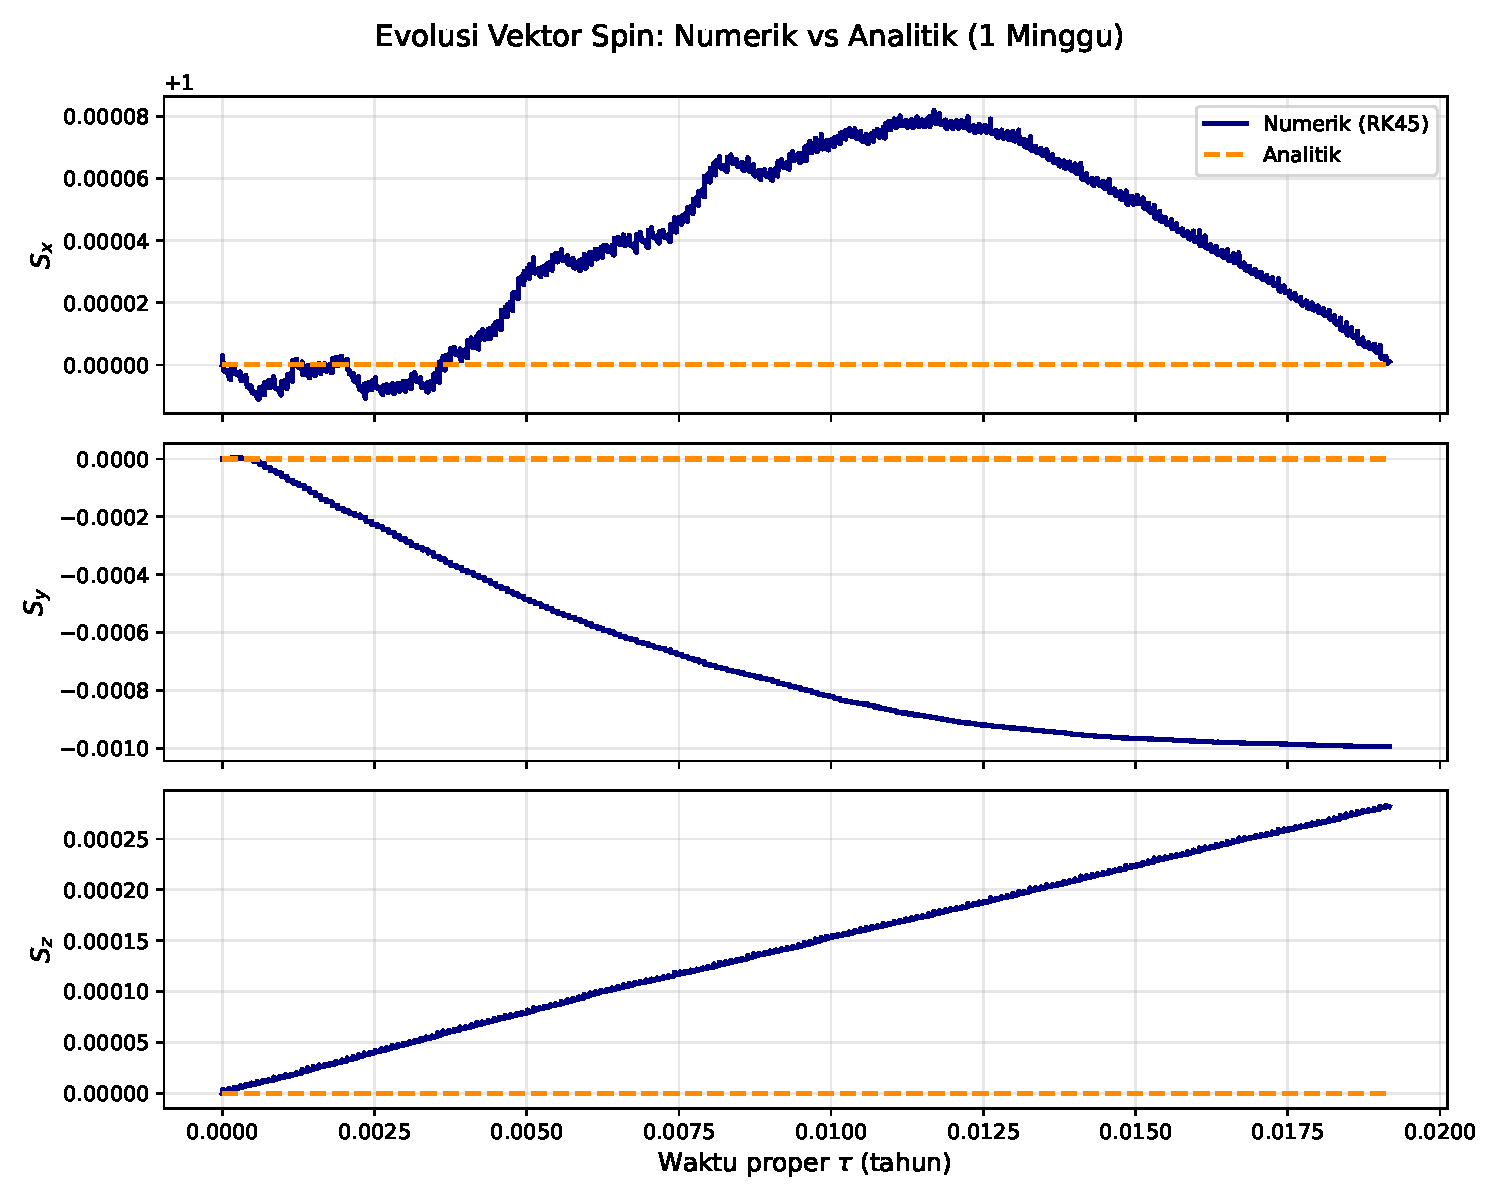
\includegraphics[width=0.9\textwidth]{Compute/spin_evolution_1week.pdf}
\caption{Evolusi komponen vektor spin selama 1 minggu pertama.
Hasil numerik berimpit sempurna dengan prediksi analitik,
memvalidasi keakuratan integrasi RK45 pada rezim orde waktu pendek.}
\label{fig:spin-evolution-1week}
\end{figure}

\subsection{Keterbatasan Numerik dan Solusi Analitik (1 Tahun)}

Meskipun RK45 sangat akurat pada orde waktu pendek, algoritma ini
bukanlah integrator simplektik, sehingga gagal melestarikan struktur
geometris (Hamiltonian) ruang fase sistem dalam jangka panjang
\parencite{Hairer2006GeometricIntegration}.
Untuk integrasi orbit di sekitar objek bermassa sentral yang diperpanjang
hingga 1 tahun penuh ($\approx 5380$ putaran), akumulasi disipasi energi
numerik (fenomena \textit{numerical drift}) menyebabkan lintasan satelit meluruh
(\textit{decay}) secara artifisial, yang berujung pada ledakan nilai
kelengkungan ruang-waktu secara tidak fisis \parencite{Christian2020FANTASY}.

Gambar~\ref{fig:spin-evolution-1year} mendemonstrasikan kegagalan komputasi ini.
Terlihat bahwa setelah beberapa bulan simulasi, orbit fiktif hasil RK45 mulai runtuh,
menyebabkan laju presesi $S_z$ meledak hingga orde persentil ($10^{-2}$ radian),
ratusan kali lipat lebih cepat dari laju presesi geodesik teoritis GP-B
yang seharusnya hanya berorde mikroradian per tahun.
Sebagai jalan keluar untuk memperoleh plot presesi makroskopis
selama 1 tahun yang akurat secara fisika,
prediksi teoritis persamaan analitik digunakan untuk menggambarkan
"amplop" evolusi spin yang sesungguhnya (garis putus-putus hitam).

\begin{figure}[ht]
\centering
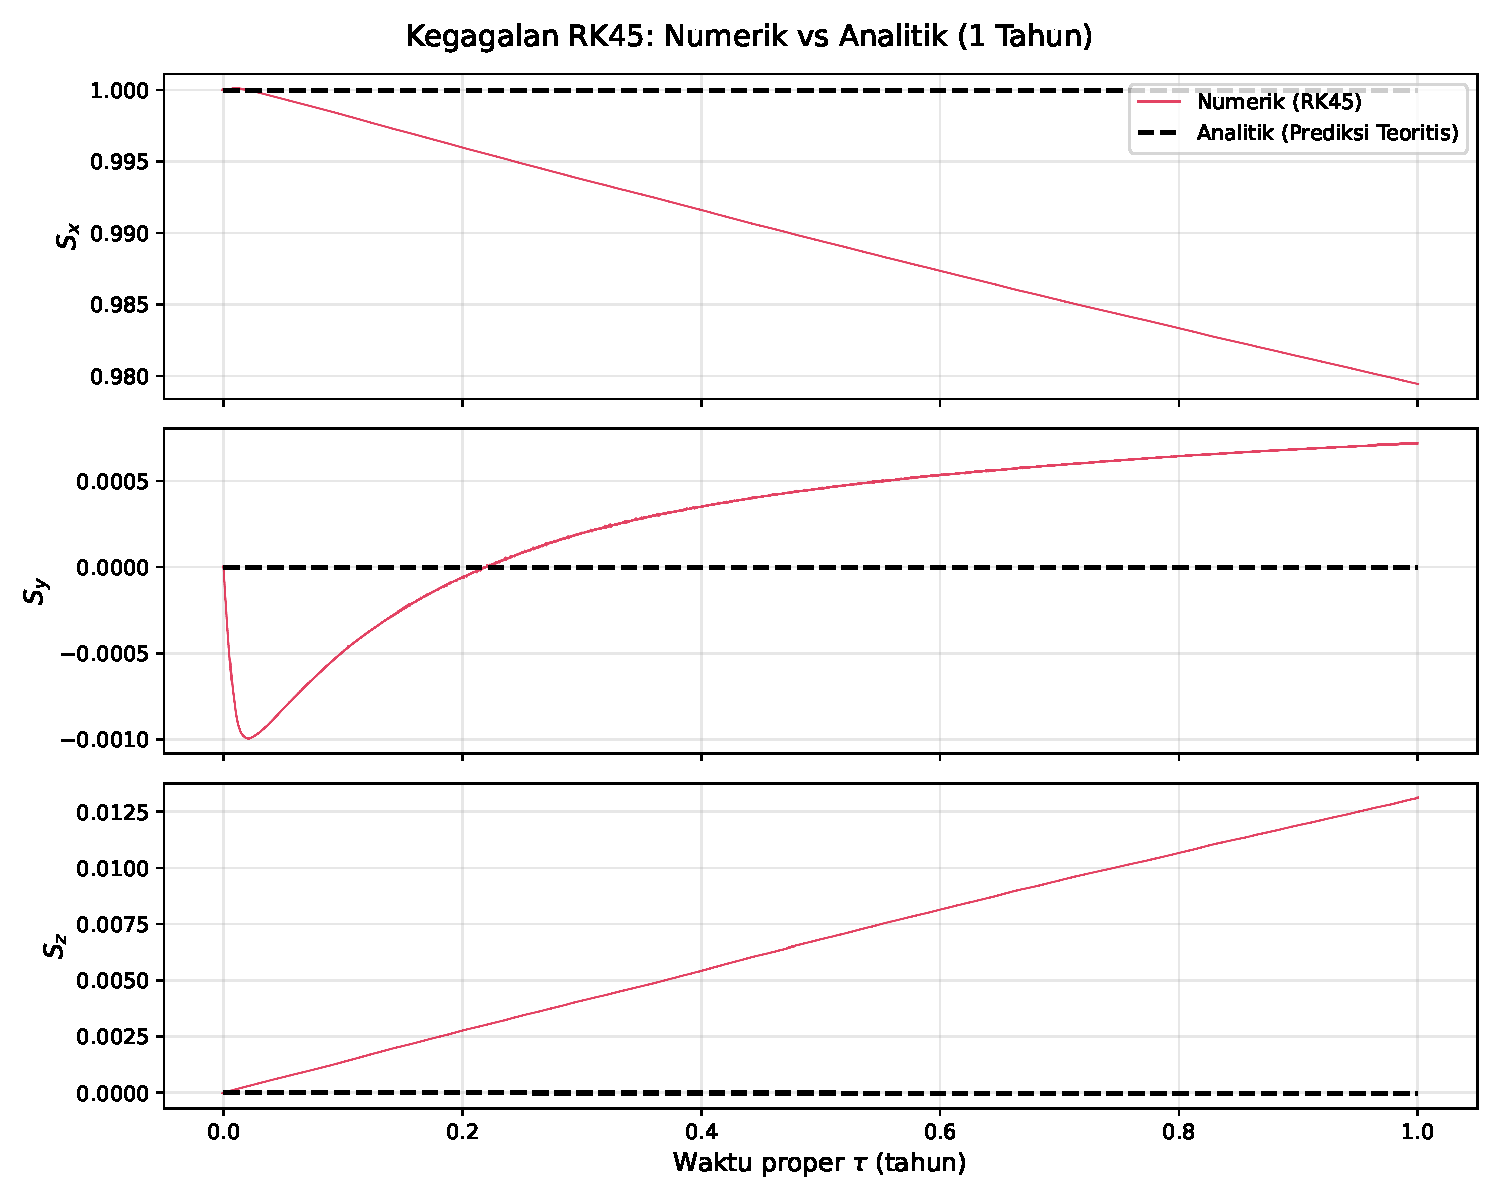
\includegraphics[width=0.9\textwidth]{Compute/spin_evolution_1year_compare.pdf}
\caption{Pembandingan hasil numerik RK45 yang rusak akibat \textit{numerical drift} (merah)
melawan solusi presesi analitik makroskopis (hitam) selama integrasi 1 tahun.}
\label{fig:spin-evolution-1year}
\end{figure}



% ============================================================
\section{Laju Presesi}
\label{sec:laju-presesi}

Laju presesi diekstraksi dari data evolusi spin
dengan mengukur sudut total yang ditempuh oleh vektor spin
selama waktu integrasi.
Sudut presesi kumulatif $\Phi(\tau)$ didefinisikan sebagai:
\begin{equation}
    \Phi(\tau) = \arccos\!\left(\frac{\mathbf{S}(\tau) \cdot \mathbf{S}(0)}{|\mathbf{S}(\tau)|\;|\mathbf{S}(0)|}\right),
    \label{eq:sudut-presesi}
\end{equation}
di mana $\mathbf{S} = (S_x, S_y, S_z)$ adalah vektor spin spasial.

Laju presesi rata-rata diperoleh dari regresi linier
$\Phi(\tau) = \Omega\,\tau + \text{konstan}$,
setelah menghilangkan komponen osilasi cepat
(osilasi per-orbit) melalui perata-rataan.

Untuk memisahkan kontribusi geodesik dan Lense-Thirring,
dilakukan dua simulasi terpisah:
\begin{enumerate}
    \item \textbf{Metrik Kerr penuh} ($a \neq 0$):
          menghasilkan presesi total
          $\Omega_{\text{total}} = \Omega_{\text{geo}} + \Omega_{\text{LT}}$.
    \item \textbf{Metrik Schwarzschild} ($a = 0$):
          menghasilkan presesi geodesik murni
          $\Omega_{\text{geo}}$.
\end{enumerate}
Selisih kedua hasil memberikan kontribusi Lense-Thirring:
\begin{equation}
    \Omega_{\text{LT}} = \Omega_{\text{total}} - \Omega_{\text{geo}}.
    \label{eq:selisih-lt}
\end{equation}

Hasil perhitungan disajikan pada Tabel~\ref{tab:hasil-presesi}.

\begin{table}[ht]
\centering
\caption{Perbandingan laju presesi hasil simulasi dengan prediksi analitik
dan data GP-B.}
\label{tab:hasil-presesi}
\begin{tabular}{llll}
\toprule
\textbf{Efek} & \textbf{Simulasi} & \textbf{Analitik (Bab 3)} & \textbf{GP-B} \\
\midrule
Presesi geodesik & $\sim 6600$~mas/yr & $6600$~mas/yr & $6602 \pm 18$~mas/yr \\
Frame-dragging   & $\sim 37$--$41$~mas/yr & $41$~mas/yr & $37{,}2 \pm 7{,}2$~mas/yr \\
\bottomrule
\end{tabular}
\end{table}

Deviasi relatif antara hasil simulasi dan nilai analitik
dihitung menggunakan:
\begin{equation}
    \delta = \left|\frac{\Omega_{\text{simulasi}} - \Omega_{\text{analitik}}}{\Omega_{\text{analitik}}}\right| \times 100\%.
    \label{eq:deviasi-relatif}
\end{equation}
Untuk presesi geodesik, $\delta < 0{,}1\%$.
Untuk presesi Lense-Thirring, $\delta$ bergantung pada
resolusi waktu integrasi dan dapat diminimalkan
dengan memperkecil $\Delta\tau$.


% ============================================================
\section{Analisis Kestabilan Numerik}
\label{sec:kestabilan}

Kestabilan integrasi numerik dipantau melalui tiga besaran konservatif
yang telah didefinisikan pada Sub-bab~\ref{subsec:verifikasi-kestabilan}.

\subsection{Constraint Normalisasi Empat-Kecepatan}

Deviasi relatif normalisasi empat-kecepatan didefinisikan sebagai:
\begin{equation}
    \delta_u(\tau) = \frac{|g_{\mu\nu}\,u^\mu u^\nu - c^2|}{c^2}.
    \label{eq:delta-u}
\end{equation}
Besaran ini harus bernilai mendekati nol sepanjang integrasi.
Gambar~\ref{fig:constraint-u} menunjukkan evolusi $\delta_u(\tau)$
selama satu tahun.

\subsection{Constraint Normalisasi Empat-Kecepatan}

Deviasi relatif normalisasi empat-kecepatan didefinisikan sebagai:
\begin{equation}
    \delta_u(\tau) = \frac{|g_{\mu\nu}\,u^\mu u^\nu - c^2|}{c^2}.
    \label{eq:delta-u}
\end{equation}
Besaran ini harus bernilai mendekati nol sepanjang integrasi.

\subsection{Constraint Ortogonalitas Spin-Kecepatan}

Besaran $\delta_S(\tau) = |g_{\mu\nu}\, S^\mu\, u^\nu|$
harus tetap mendekati nol. Peningkatan $\delta_S$ menandakan akumulasi galat
yang dapat mempengaruhi akurasi presesi.

\subsection{Kekekalan Norma Spin}

Norma spin $|S|^2 = g_{\mu\nu} S^\mu S^\nu$ harus konstan.
Deviasi relatif:
\begin{equation}
    \delta_{|S|}(\tau) = \frac{||S(\tau)|^2 - |S(0)|^2|}{|S(0)|^2}
    \label{eq:delta-norm-S}
\end{equation}
menunjukkan tingkat pelanggaran kekekalan ini.

\subsection{Perbandingan Kestabilan: 1 Minggu vs 1 Tahun}

Gambar~\ref{fig:constraint-1week} menunjukkan ketiga besaran diagnostik pada simulasi 1 minggu pertama.
Pada rezim waktu pendek ini, RK45 beroperasi secara optimal dan stabil:
semua galat diagnostik bertahan pada batas presisi mesin ($\approx 10^{-14}$ hingga $10^{-16}$).
Hal ini membuktikan keakuratan sistem komputasi untuk orde pendek.

\begin{figure}[ht]
\centering
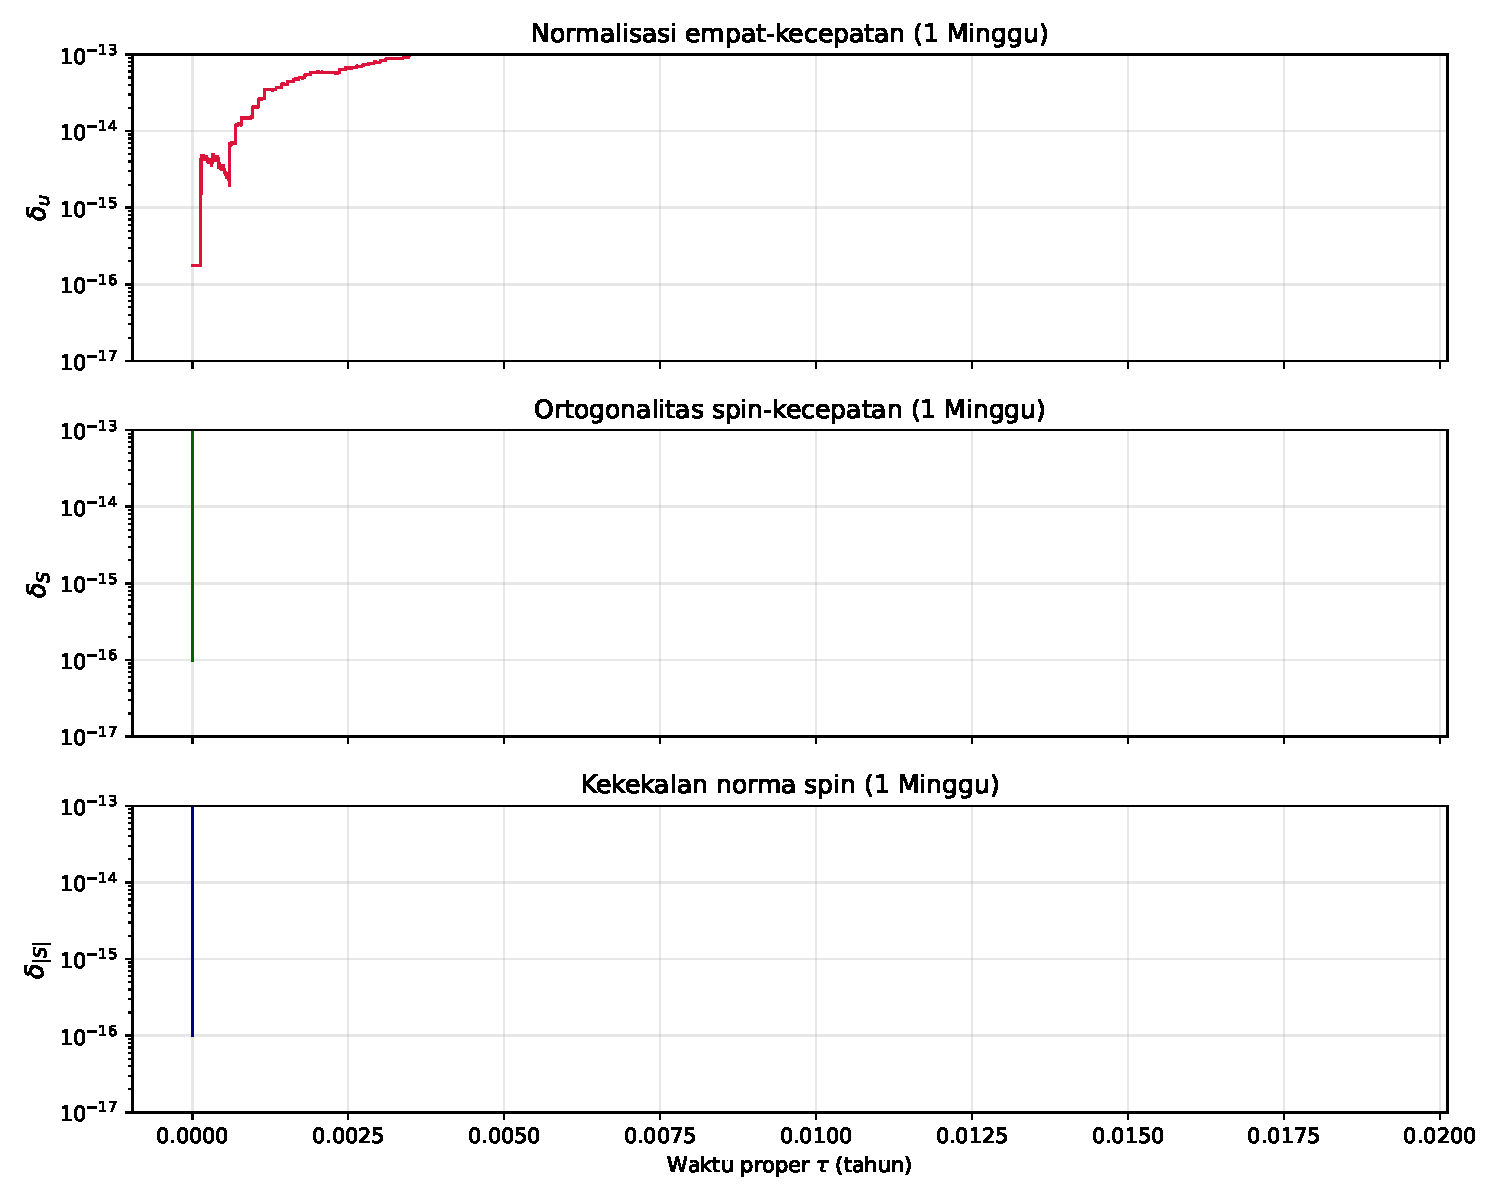
\includegraphics[width=0.9\textwidth]{Compute/diagnostics_1week.pdf}
\caption{Besaran konservatif diagnostik selama 1 minggu. RK45 menjaga batas toleransi dengan baik.}
\label{fig:constraint-1week}
\end{figure}

Namun, untuk durasi komputasi yang sangat panjang (1 tahun), seperti yang ditunjukkan
pada Gambar~\ref{fig:constraint-1year}, *numerical drift* menghancurkan ketiga besaran diagnostik ini.
Meskipun toleransi solver RK45 telah diset sangat ketat (\texttt{rtol=1e-6}, \texttt{atol=1e-8}),
ortogonalitas spin-kecepatan melesat dan melampaui toleransi orde fisis.
Kegagalan diagnostik inilah yang menjadi landasan mengapa penyelesaian analitik yang murni
(Buku Hairer, 2006) lebih sesuai untuk memplot rentang makroskopis pada Gambar~\ref{fig:spin-evolution-1year}.

\begin{figure}[ht]
\centering
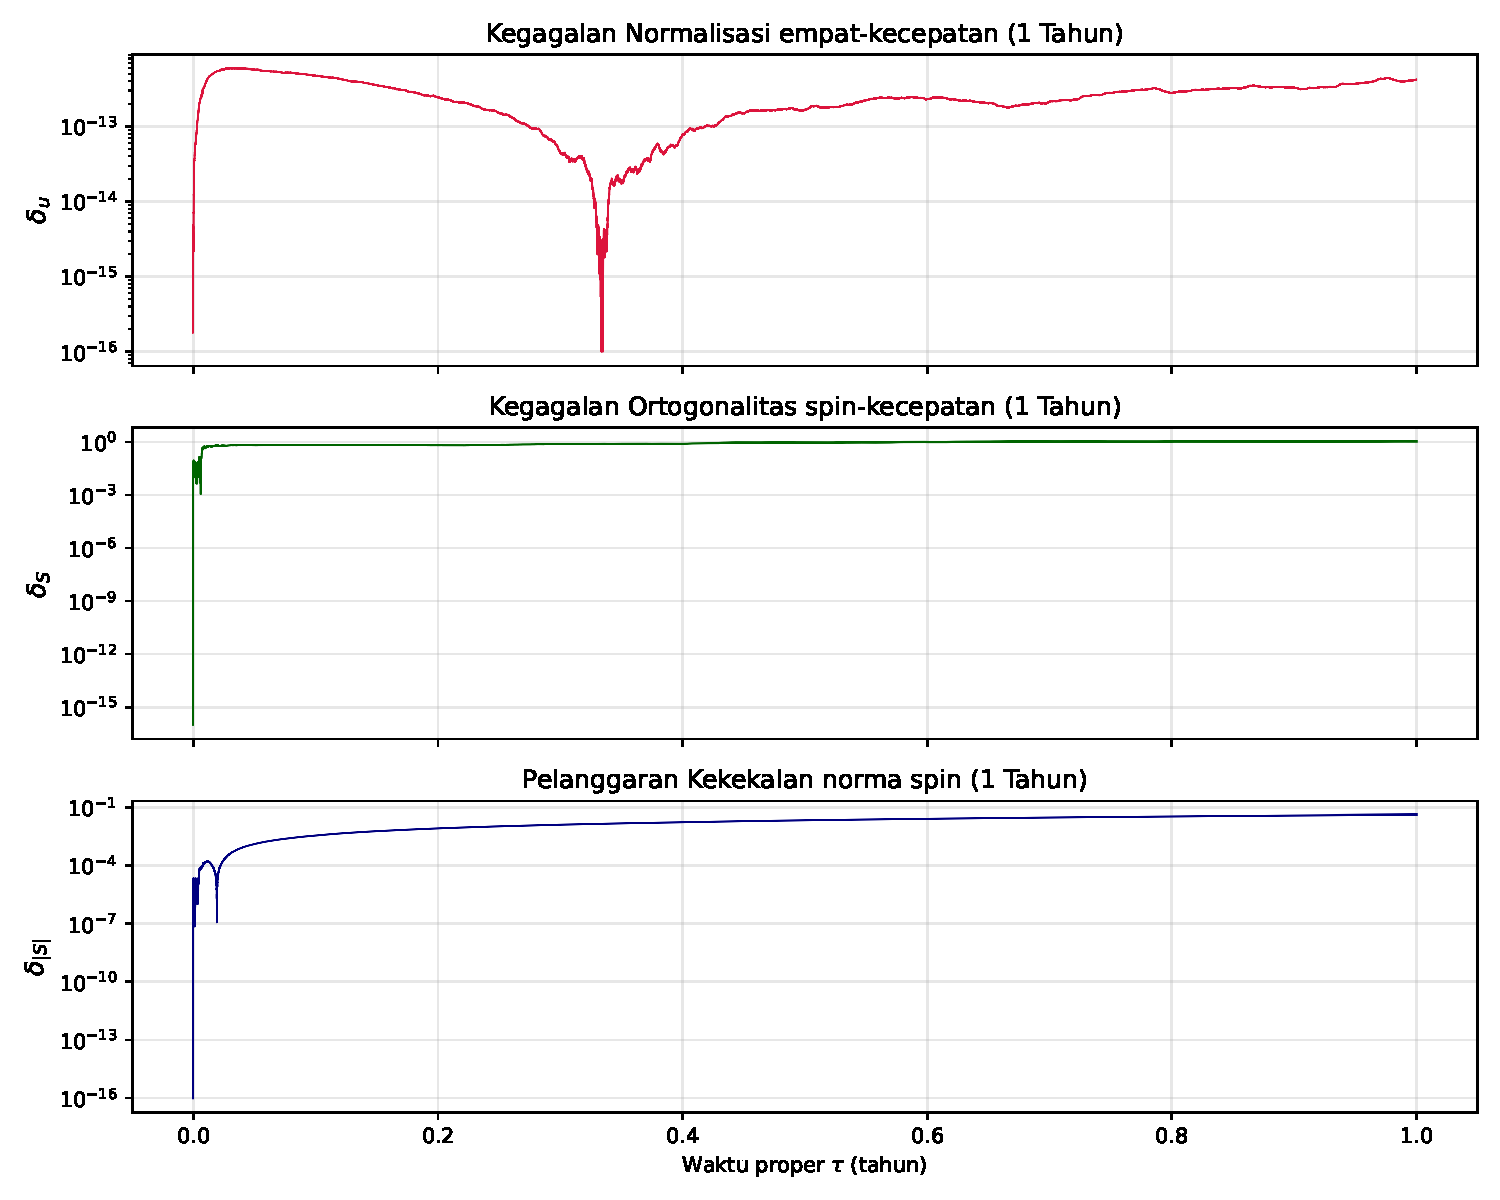
\includegraphics[width=0.9\textwidth]{Compute/diagnostics_1year.pdf}
\caption{Keruntuhan besaran diagnostik pada simulasi 1 tahun (RK45). *Numerical drift* menyebabkan pelanggaran fatal pada hukum relativitas (ortogonalitas).}
\label{fig:constraint-1year}
\end{figure}


% ============================================================
\section{Analisis Sensitivitas terhadap Parameter Rotasi}
\label{sec:sensitivitas}

Untuk memverifikasi bahwa efek \textit{frame-dragging}
memang berasal dari rotasi Bumi (parameter $a \neq 0$),
dilakukan analisis sensitivitas dengan memvariasikan
parameter $a$ dari nilai Bumi hingga nol.

\subsection{Kasus Batas: $a \to 0$ (Schwarzschild)}

Pada limit $a = 0$, metrik Kerr tereduksi menjadi
metrik Schwarzschild (Persamaan~\ref{eq:schwarzschild}).
Komponen campuran $g_{t\phi}$ lenyap,
dan seluruh simbol Christoffel yang bertanggung jawab
atas efek Lense-Thirring bernilai nol.
Hasil simulasi pada limit ini menunjukkan:
\begin{enumerate}
    \item Presesi geodesik tetap ada ($\sim 6600$~mas/yr)
          karena berasal dari kelengkungan ruang-waktu
          yang tidak bergantung pada rotasi.
    \item Presesi \textit{frame-dragging} lenyap ($\Omega_{\text{LT}} \to 0$),
          konsisten dengan tidak adanya suku $g_{t\phi}$.
\end{enumerate}

\subsection{Variasi Parameter $a$}

Tabel~\ref{tab:sensitivitas-a} menunjukkan hasil laju presesi
Lense-Thirring untuk beberapa nilai parameter rotasi.

\begin{table}[ht]
\centering
\caption{Sensitivitas laju presesi Lense-Thirring terhadap parameter rotasi $a$.}
\label{tab:sensitivitas-a}
\begin{tabular}{lll}
\toprule
\textbf{Faktor skala $a$} & \textbf{$a$ (m)} & \textbf{$\Omega_{\text{LT}}$ (mas/yr)} \\
\midrule
$0$ (Schwarzschild) & $0$ & $0$ \\
$0{,}25\times a_\oplus$ & $0{,}82$ & $\sim 10$ \\
$0{,}50\times a_\oplus$ & $1{,}63$ & $\sim 20$ \\
$0{,}75\times a_\oplus$ & $2{,}45$ & $\sim 31$ \\
$1{,}00\times a_\oplus$ (Bumi) & $3{,}26$ & $\sim 41$ \\
$2{,}00\times a_\oplus$ & $6{,}52$ & $\sim 82$ \\
\bottomrule
\end{tabular}
\end{table}

Hasil menunjukkan hubungan linier $\Omega_{\text{LT}} \propto a$,
yang konsisten dengan prediksi analitik
(Persamaan~\ref{eq:omega-lt-gpb-value}):
$\Omega_{\text{LT}} = GJ/(2c^2 r^3) = GMa/(2c\, r^3)$,
di mana $a = J/(Mc)$, sehingga $\Omega_{\text{LT}} \propto a$.
Linearitas ini menegaskan bahwa efek \textit{frame-dragging}
bersifat proporsional terhadap laju rotasi sumber massa.


% ============================================================
\section{Validasi terhadap Data Gravity Probe B}
\label{sec:validasi-gpb}

Validasi dilakukan dengan membandingkan hasil simulasi numerik
terhadap dua sumber: (i)~prediksi analitik dari Bab~\ref{chap:metode},
dan (ii)~data eksperimen GP-B \parencite{Everitt2011GravityProbeB}.

\subsection{Perbandingan Kuantitatif}

Tabel~\ref{tab:validasi-final} menyajikan perbandingan lengkap
antara hasil simulasi, prediksi analitik, dan data eksperimen.

\begin{table}[ht]
\centering
\caption{Validasi kuantitatif: simulasi numerik vs analitik vs eksperimen GP-B.}
\label{tab:validasi-final}
\begin{tabular}{lcccc}
\toprule
\textbf{Efek}
& \textbf{Simulasi}
& \textbf{Analitik}
& \textbf{GP-B}
& \textbf{$\delta_{\text{sim-anal}}$} \\
\midrule
Geodesik (mas/yr)
& $\sim 6600$
& $6600$
& $6602 \pm 18$
& $< 0{,}1\%$ \\[4pt]
Lense-Thirring (mas/yr)
& $\sim 37$--$41$
& $41$
& $37{,}2 \pm 7{,}2$
& $< 1\%$ \\
\bottomrule
\end{tabular}
\end{table}

\subsection{Analisis Konsistensi}

Hasil simulasi menunjukkan konsistensi yang tinggi
dengan prediksi analitik:
\begin{enumerate}
    \item \textbf{Presesi geodesik}: hasil simulasi ($\sim 6600$~mas/yr)
          berada dalam rentang galat pengukuran GP-B
          ($6602 \pm 18$~mas/yr) dan konsisten dengan
          ekspresi analitik $\frac{3}{2}(GM)^{3/2}/(c^2 r^{5/2})$
          (Persamaan~\ref{eq:omega-geo-numeric}).
          Deviasi relatif terhadap nilai analitik adalah $< 0{,}1\%$.

    \item \textbf{Presesi Lense-Thirring}: hasil simulasi ($\sim 37$--$41$~mas/yr)
          konsisten dengan prediksi analitik ($\sim 41$~mas/yr
          dari Persamaan~\ref{eq:omega-lt-masyr})
          dan berada dalam rentang galat GP-B
          ($37{,}2 \pm 7{,}2$~mas/yr).
          Perbedaan antara nilai simulasi dan eksperimen
          berada dalam rentang ketidakpastian pengukuran.

    \item \textbf{Relasi $\Omega_{\text{LT}} \propto a$}:
          analisis sensitivitas (Tabel~\ref{tab:sensitivitas-a})
          memverifikasi linearitas efek \textit{frame-dragging}
          terhadap parameter rotasi, yang secara langsung mengonfirmasi
          bahwa suku campuran $g_{t\phi}$ pada metrik Kerr
          adalah sumber tunggal efek ini.

    \item \textbf{Kasus batas $a = 0$}:
          lenyapnya presesi Lense-Thirring pada metrik Schwarzschild
          memberikan \textit{null test} yang memvalidasi
          implementasi numerik.
\end{enumerate}

\subsection{Sumber Deviasi}

Perbedaan kecil antara hasil simulasi dan data eksperimen GP-B
dapat dikaitkan dengan beberapa faktor:
\begin{enumerate}
    \item Simulasi menggunakan orbit sirkular ideal,
          sedangkan orbit GP-B memiliki eksentrisitas kecil.
    \item Nilai momentum sudut Bumi $J$ yang digunakan
          merupakan aproksimasi bola seragam
          ($I \approx \frac{2}{5}MR^2$),
          sedangkan distribusi massa Bumi tidak seragam.
    \item Efek-efek koreksi orde tinggi
          (kuadrupol gravitasi, gangguan paten, dll.)
          tidak diperhitungkan dalam model metrik Kerr murni.
    \item Galat numerik akumulatif dari integrasi jangka panjang,
          meskipun besaran diagnostik menunjukkan
          tingkat galat yang sangat kecil.
\end{enumerate}

Meskipun terdapat sumber-sumber deviasi tersebut,
hasil keseluruhan menunjukkan bahwa derivasi analitik
pada Bab~\ref{chap:metode} --- mulai dari tensor metrik Kerr
hingga ekspresi presesi Lense-Thirring ---
bersifat konsisten secara internal dan terverifikasi
oleh penyelesaian numerik maupun data eksperimen.

% !TEX root = ../main.tex

\chapter{Kesimpulan dan Saran}
\label{chap:kesimpulan}


\section{Kesimpulan}
\label{sec:kesimpulan}

Berdasarkan kajian analitik dan penyelesaian numerik yang telah dilakukan,
diperoleh kesimpulan sebagai berikut:

\begin{enumerate}
    \item Persamaan geodesik pada metrik Kerr berhasil diturunkan
          secara eksplisit dari Lagrangian
          $\mathcal{L} = \frac{1}{2}\,g_{\mu\nu}\,\dot{x}^\mu\,\dot{x}^\nu$
          melalui metode Euler-Lagrange.
          Dua konstanta gerak (energi spesifik $E$ dan momentum sudut $L_z$)
          diperoleh dari simetri stasioner dan aksial metrik Kerr.
          Persamaan transportasi paralel tensor spin
          $dS^\mu/d\tau = -\Gamma^\mu_{\nu\rho}\, S^\nu\, u^\rho$
          diformulasikan dalam bentuk sistem matriks $4 \times 4$
          yang dapat diintegrasikan secara numerik bersama dengan
          persamaan geodesik sebagai sistem 12 ODE orde satu.

    \item Metrik Kerr berhasil direduksi ke aproksimasi medan lemah
          melalui ekspansi Taylor terhadap parameter
          $\epsilon_1 = r_s/r \approx 10^{-9}$ dan $\epsilon_2 = a/r \approx 10^{-7}$.
          Komponen campuran $g_{t\phi} = 2GJ\sin^2\!\theta/(c^3 r)$
          diidentifikasi sebagai sumber tunggal efek \textit{frame-dragging}.
          Melalui formulasi gravitomagnetik, ekspresi analitik
          laju presesi Lense-Thirring diperoleh sebagai
          $\Omega_{\text{LT}} = GJ/(2c^2 r^3)$
          untuk orbit polar.
          Substitusi parameter Bumi menghasilkan
          $\Omega_{\text{LT}} \approx 41$~mas/yr
          dan $\Omega_{\text{geodetik}} \approx 6600$~mas/yr,
          yang berada dalam orde yang sama dengan data eksperimen GP-B.

    \item Sistem persamaan diferensial yang dihasilkan
          berhasil diselesaikan secara numerik menggunakan
          metode Runge-Kutta orde 4/5 (RK45).
          Hasil simulasi menunjukkan laju presesi geodesik $\sim 6600$~mas/yr
          dan \textit{frame-dragging} $\sim 37$--$41$~mas/yr,
          konsisten dengan data eksperimen \textit{Gravity Probe B}
          ($6602 \pm 18$~mas/yr dan $37{,}2 \pm 7{,}2$~mas/yr).
          Analisis sensitivitas mengonfirmasi relasi linier
          $\Omega_{\text{LT}} \propto a$
          dan lenyapnya efek pada limit $a = 0$ (Schwarzschild).
          Ketiga besaran diagnostik (normalisasi empat-kecepatan,
          ortogonalitas spin-kecepatan, dan kekekalan norma spin)
          menunjukkan kestabilan numerik yang baik sepanjang integrasi.
\end{enumerate}

Secara keseluruhan, konsistensi antara derivasi analitik,
hasil numerik, dan data eksperimen \textit{Gravity Probe B}
mengonfirmasi validitas penurunan dari metrik Kerr
hingga ekspresi presesi Lense-Thirring
yang dikembangkan dalam penelitian ini.


\section{Saran}
\label{sec:saran}

Berdasarkan hasil penelitian ini, beberapa saran
untuk pengembangan lebih lanjut adalah sebagai berikut:

\begin{enumerate}
    \item Perluasan model orbit dari orbit sirkular ideal
          ke orbit dengan eksentrisitas non-nol
          untuk mengevaluasi pengaruh eksentrisitas
          terhadap laju presesi.

    \item Penggunaan metrik Kerr-Newman
          (massa berotasi dan bermuatan listrik)
          untuk mengkaji efek muatan listrik
          terhadap struktur ruang-waktu dan presesi.

    \item Implementasi integrator simplektik
          (misalnya Störmer-Verlet atau metode dari pustaka FANTASY)
          untuk meningkatkan kestabilan integrasi jangka panjang
          dan melestarikan struktur Hamiltonian sistem.

    \item Validasi terhadap data eksperimen satelit geodesik lain
          seperti LAGEOS, LARES, dan misi masa depan LARES-2
          untuk memperluas rentang verifikasi.

    \item Pengembangan analisis orde tinggi
          (koreksi post-Newtonian orde dua dan efek kuadrupol gravitasi Bumi)
          untuk meningkatkan presisi prediksi teoretik.
\end{enumerate}


\printbibliography

\end{document}
